

\documentclass[12pt]{article}
\usepackage{subfig}
\usepackage[english]{babel}
\usepackage[utf8x]{inputenc}
\usepackage[T1]{fontenc}
\usepackage{amsmath}
\usepackage{graphicx}
\usepackage{pstricks,pst-node}
\usepackage{stmaryrd}
\usepackage{gastex}
\usepackage{comment}
\usepackage{xcolor}
\usepackage{listings}
\usepackage{float}
\usepackage{url}
\usepackage[margin=1.3in]{geometry}




\catcode`\_=12

\definecolor{mGreen}{rgb}{0,0.6,0}
\definecolor{mGray}{rgb}{0.5,0.5,0.5}
\definecolor{mPurple}{rgb}{0.58,0,0.82}
\definecolor{backgroundColour}{rgb}{0.95,0.95,0.92}

\lstdefinestyle{CStyle}{
    backgroundcolor=\color{backgroundColour},   
    commentstyle=\color{mGreen},
    keywordstyle=\color{magenta},
    numberstyle=\tiny\color{mGray},
    stringstyle=\color{mPurple},
    basicstyle=\footnotesize,
    breakatwhitespace=false,         
    breaklines=true,                 
    captionpos=b,                    
    keepspaces=true,                 
    numbers=left,                    
    numbersep=5pt,                  
    showspaces=false,                
    showstringspaces=false,
    showtabs=false,                  
    tabsize=2,
    language=C
}




\usepackage[colorinlistoftodos]{todonotes}
\usepackage{wrapfig}

\begin{document}

\begin{titlepage}

\newcommand{\HRule}{\rule{\linewidth}{0.5mm}} % Defines a new command for the horizontal lines, change thickness here

\center % Center everything on the page
 
%----------------------------------------------------------------------------------------
%	HEADING SECTIONS
%----------------------------------------------------------------------------------------


\textsc{\Large Projet de recherche}\\[0.5cm] % Major heading such as course name
\textsc{\large "LU3IN013"}\\[0.5cm] % Minor heading such as course title

%----------------------------------------------------------------------------------------
%	TITLE SECTION
%----------------------------------------------------------------------------------------

\HRule \\[0.4cm]
{\huge \bfseries Système de vision temps réel pour drones}\\[0.4cm] % Title of your document
\HRule \\[1.5cm]
 
%----------------------------------------------------------------------------------------
%	AUTHOR SECTION
%----------------------------------------------------------------------------------------

\begin{minipage}{0.4\textwidth}
\begin{flushleft} \large
\emph{Equipe:}\\~\\

Johan-Luca \textsc{Rossi}\\
Qingyuan \textsc{Yao}\\
Lina \textsc{Saichi}\\
Mohamed \textsc{Meziane}\\
Melissa \textsc{Larbi}\\
Syrine \textsc{Marzougui}\\
% Your name
\end{flushleft}
\end{minipage}
~
\begin{minipage}{0.4\textwidth}
\begin{flushright} \large
\emph{Encadrants:} \\~\\
Fabrice \textsc{Kordon}\\ % Supervisor's Name
Lionel \textsc{Lacassagne}\\~\\~\\~\\~\\
\end{flushright}
\end{minipage}\\[2cm]

% If you don't want a supervisor, uncomment the two lines below and remove the section above
%\Large \emph{Author:}\\
%John \textsc{Smith}\\[3cm] % Your name

%----------------------------------------------------------------------------------------
%	DATE SECTION
%----------------------------------------------------------------------------------------

 % Date, change the \today to a set date if you want to be precise

%----------------------------------------------------------------------------------------
%	LOGO SECTION
%----------------------------------------------------------------------------------------


\includegraphics[scale=0.5]{logo.png}\\[1cm] % Include a department/university logo - this will require the graphicx package
 
%----------------------------------------------------------------------------------------

\vfill % Fill the rest of the page with whitespace

\end{titlepage}




%DEBUT DU DOC 
\topskip0pt
\vspace*{\fill}

\begin{center}
    \textbf{\Large Remerciements}
    \\~\\~\\
\end{center}
Avant tout, nous tenons à remercier monsieur Fabrice KORDON et monsieur Lionel LACASSAGNE pour nous avoir sélectionnés et fait confiance pour ce projet, pour le temps investi et la patience dont ils ont fait preuve durant notre encadrement qui fut d'une grande qualité.\\ 
Ce projet nous a permis d'appréhender l'ampleur qu'un projet informatique pouvait avoir et la rigueur nécessaire à son bon déroulement et au travail en équipe. Enfin, les précieux conseils et le savoir que nous on transmis nos encadrant nous aura permis de devenir de meilleurs informaticiens.
\vspace*{\fill}

\newpage

\renewcommand{\contentsname}{Sommaire}
\tableofcontents
\newpage

\section{Introduction}

\subsection{Contexte}
 Dans le cadre de l’unité d’enseignement LU3IN013 , nous participons à la réalisation d’un projet intitulé “Système de vision temps réel pour drone”. Ce document présente le rapport final du projet dont le but est d’expliquer les solutions adoptées pour faire face aux nombreux problèmes rencontrés et atteindre les objectifs demandés.

\subsection{Présentation du projet}
 Ce projet consiste à implémenter un programme sur ordinateur (sous Ubuntu 18.04), qui ne sera pas embarqué sur le drone, dont le but est de conférer une capacité d'autonomie au drone pour détecter une mire à proximité, puis de voler et atterrir à une distance suffisamment proche. Le drone utilisé est un Parrot Bebop 2 \cite{bebop}.

\subsection{Objectif}
L’objectif de ce projet est d'étudier des méthodes simples non basées sur l'apprentissage profond (pour des raisons de performances), dans le but de récupérer le flux vidéo du drone, décomposer ce flux en images que l'on traite pour trouver les coordonnées de la mire et ensuite à l'aide de ces coordonnées, estimer la position du drone par rapport à la mire et lui envoyer la commande la plus adaptée pour le ramener à l’emplacement voulu. L’objectif était aussi d’intégrer des exigences de complexité (temps de calcul) pour assurer un traitement en temps réel.

\section{Architecture}

\subsection{Principe de fonctionnement\label{principe}}
Ce projet est divisé en 3 partie:
\begin{itemize}
    \item Partie Pilotage: initialisation du programme et communication avec le drone (connexion au WiFi, récupération du flux, envoie des commandes)
    \item Partie Bas-niveau: découpage du flux, analyse des images pour trouver les positions des 4 hirondelles
    \item Partie Haut-niveau: déduction de la position spatiale à partir des positions des hirondelles 
    
    Au début du programme, après l'initiation du Pilotage et la création du flux, la partie bas-niveau (cf. Section \ref{bas}) est appelée pour lancer une boucle événementielle, celle-ci extrait l'image depuis le flux, initialement 24 fois par seconde mais pour des raisons de performance (cf. Section \ref{bas}) 12 fois par seconde . A partir de chaque image, une analyse est faite pour trouver les positions des 4 hirondelles de la mire (cf. Figure \ref{fig:mire}), ces positions sont ensuite passées à la partie haut-niveau pour déduire la position spatiale du drone par rapport à la mire. Ayant fait la déduction, la partie haut-niveau appelle la fonction de callback de la partie Pilotage, pour qu'elle puisse envoyer la commande au drone selon la déduction de la partie haut\_niveau. Cette séquence d'analyse et d'exécution depuis la boucle est bien sûr appelée 12 fois par seconde, pour un pilotage réactif et précis. Voir Figure \ref{fig:fct} pour un résumé de l'exécution.
    \begin{figure}[H]
    \centering
    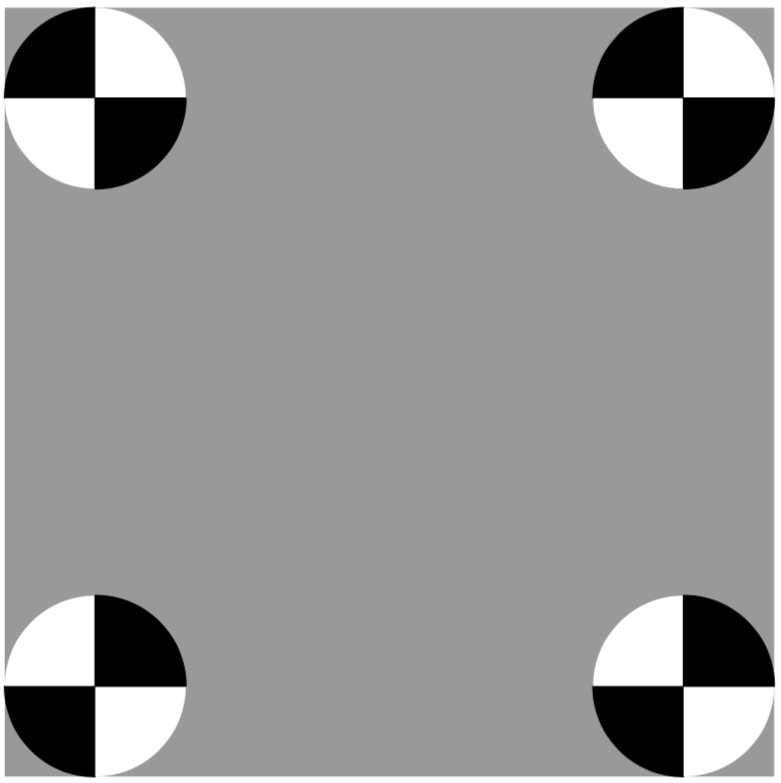
\includegraphics[width=2cm]{mire.png}
    \caption{La mire et ses quatre hirondelles}
    \label{fig:mire}
    \end{figure}
    %A part du fonctionnement principal, des mécanismes ont été mis en places pour garantir le bon fonctionnement du programme et la sécurité du drone. (cf. 3.4)
\end{itemize}
\begin{figure}[H]
\centering
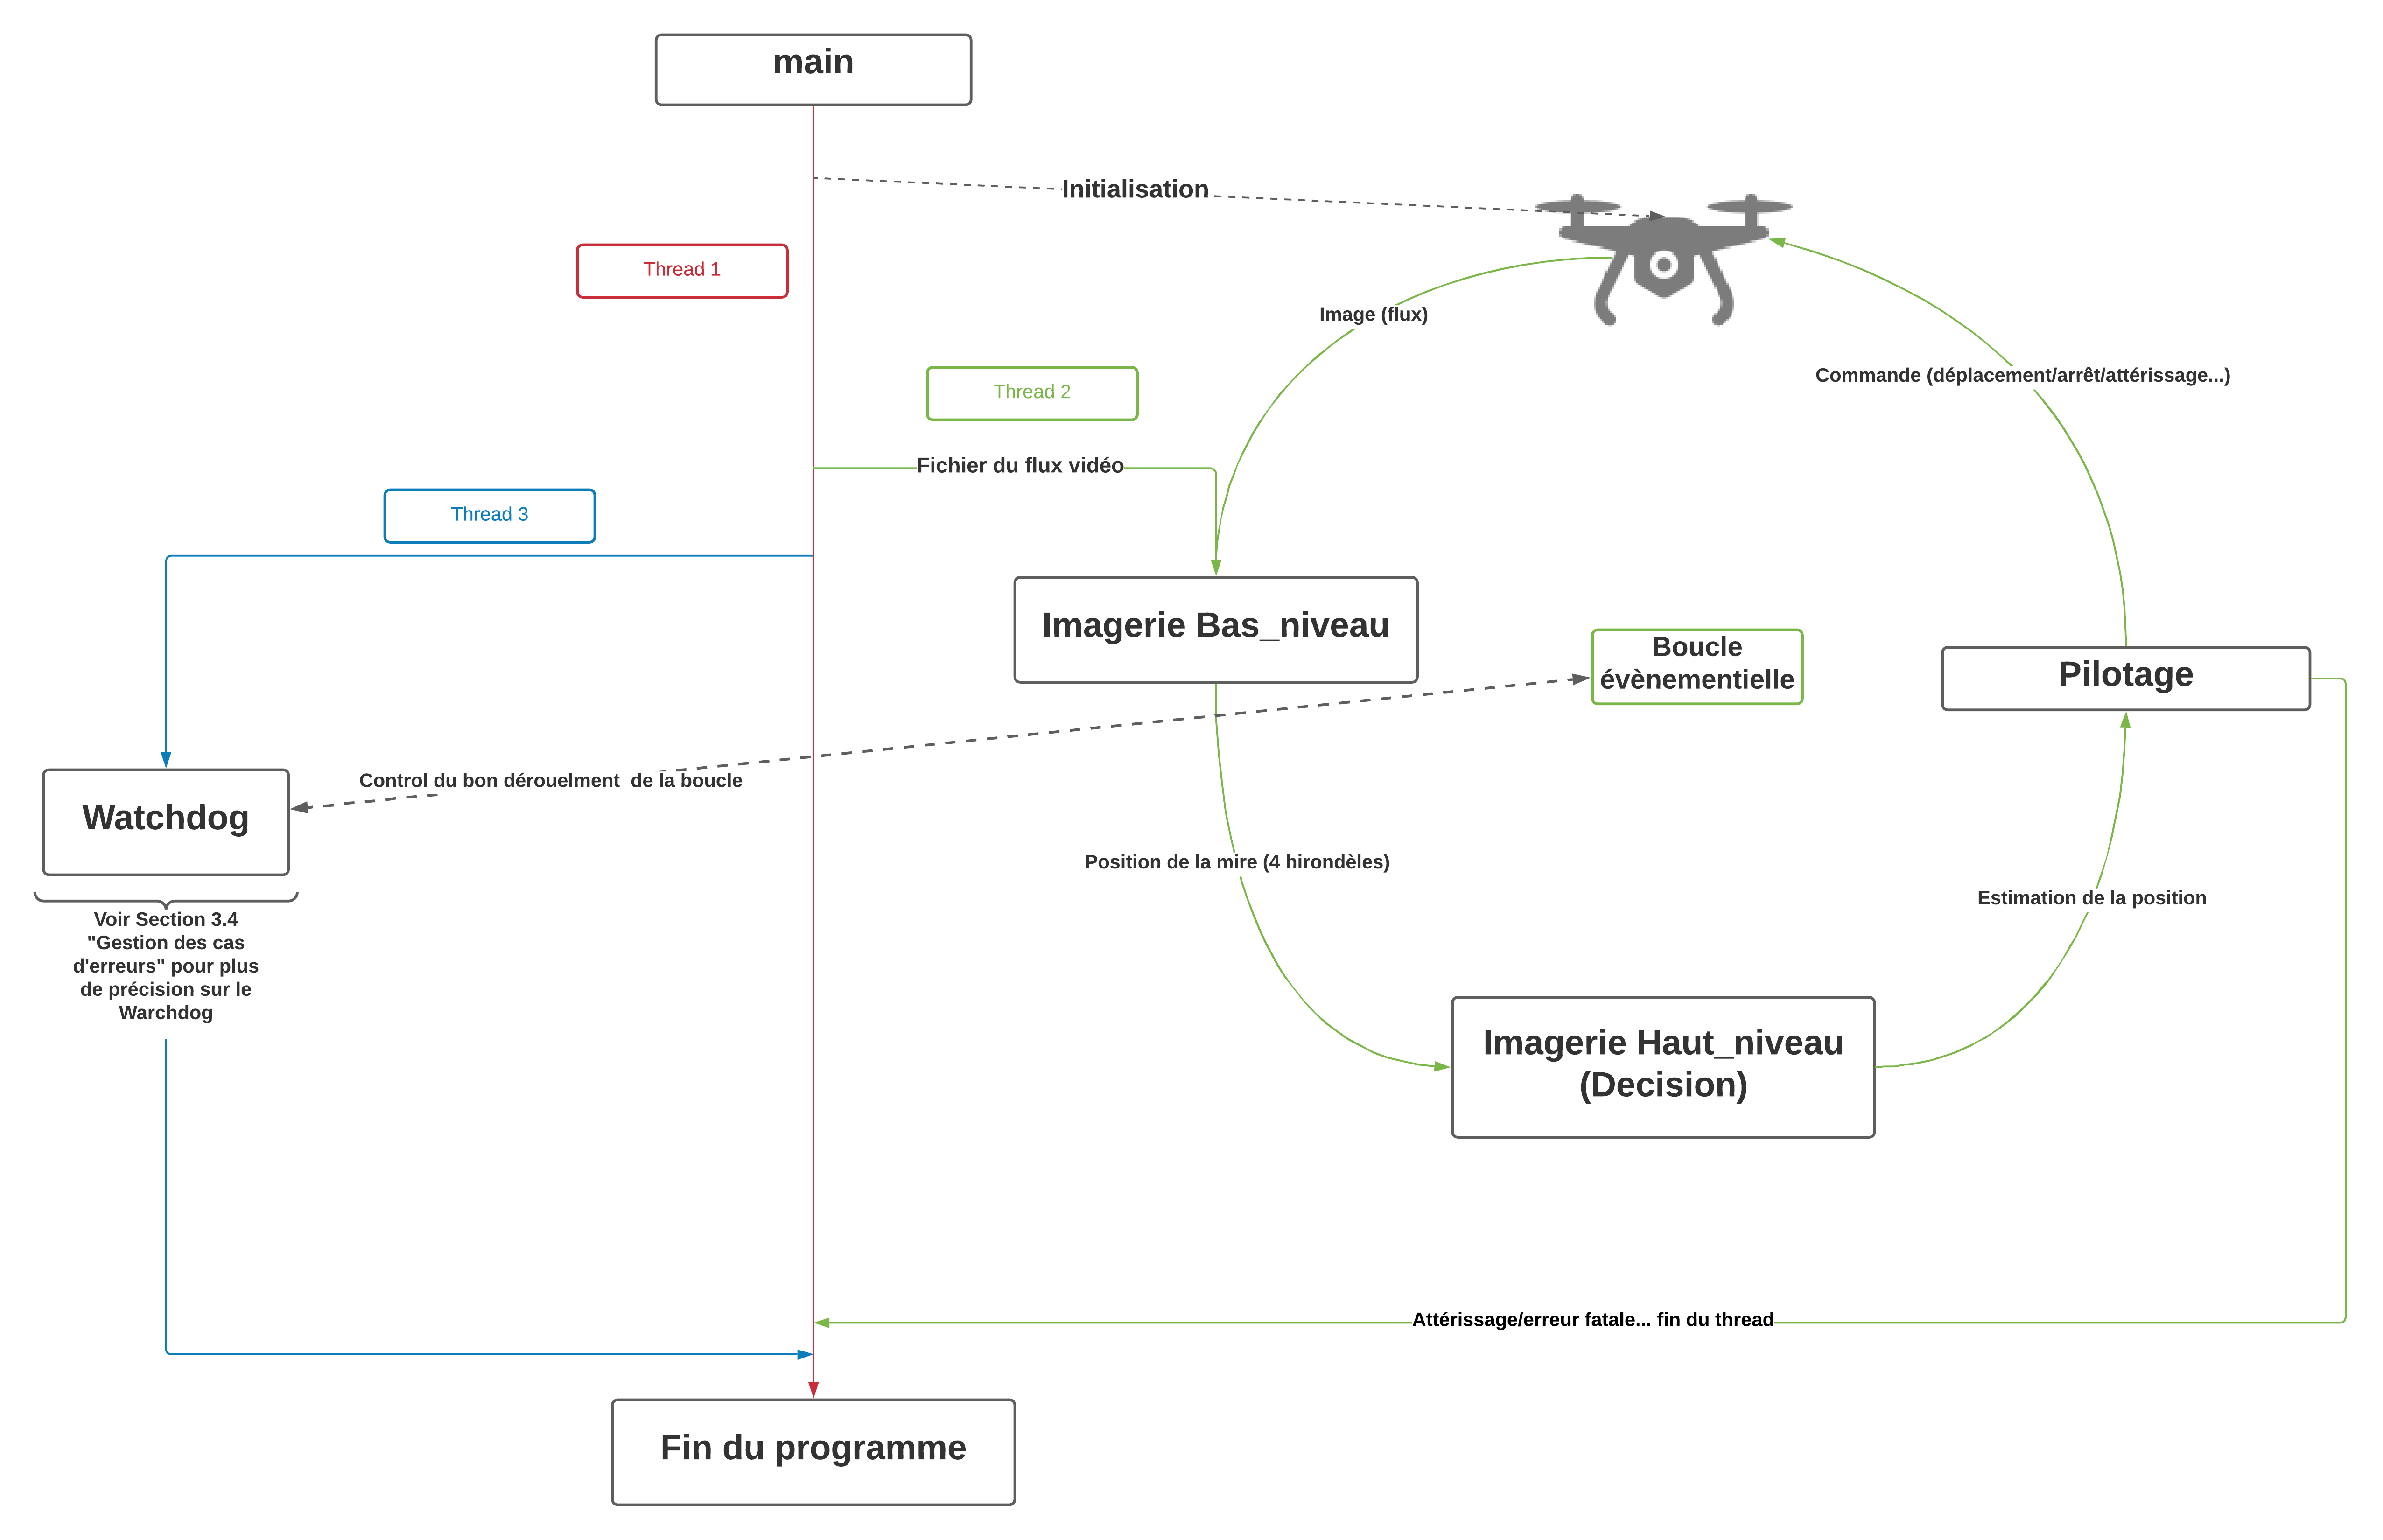
\includegraphics[width=15cm]{Fonctionnement_simple.png}
\caption{Principe de fonctionnement}
\label{fig:fct}
\end{figure}
Le programme s'occupe de l'écriture et la lecture du flux en même temps, il faut donc forcément gérer ce parallélisme, nous faisons cela avec des threads (cf. Figure \ref{fig:fct}). Les pthreads (POSIX threads\cite{pthreads}) permettent d'avoir plusieurs exécutions en parallèle en partagent les ressources, ce qui nous permet de modifier les variables globales.
La boucle événementielle qui s'occupe de la lecture du flux sera appelée dans un pthread pendant que l'écriture reste dans le thread principal. Les 2 threads se parlent avec un fichier du flux (cf. Section 3.2).

\subsection{Architecture du projet}
Nous avons développé sur GIT, hébergé sur gitHub\cite{github} , on peux y retrouver le code source\cite{git} et l'historique de nos avancement. La Figure \ref{fig:archi} représente principalement le GIT, il ne contient pas l'exécutable, c'est à travers l'API de Parrot que celui-ci sera généré (cf. Section \ref{compi}).
\begin{figure}[H]
\centering
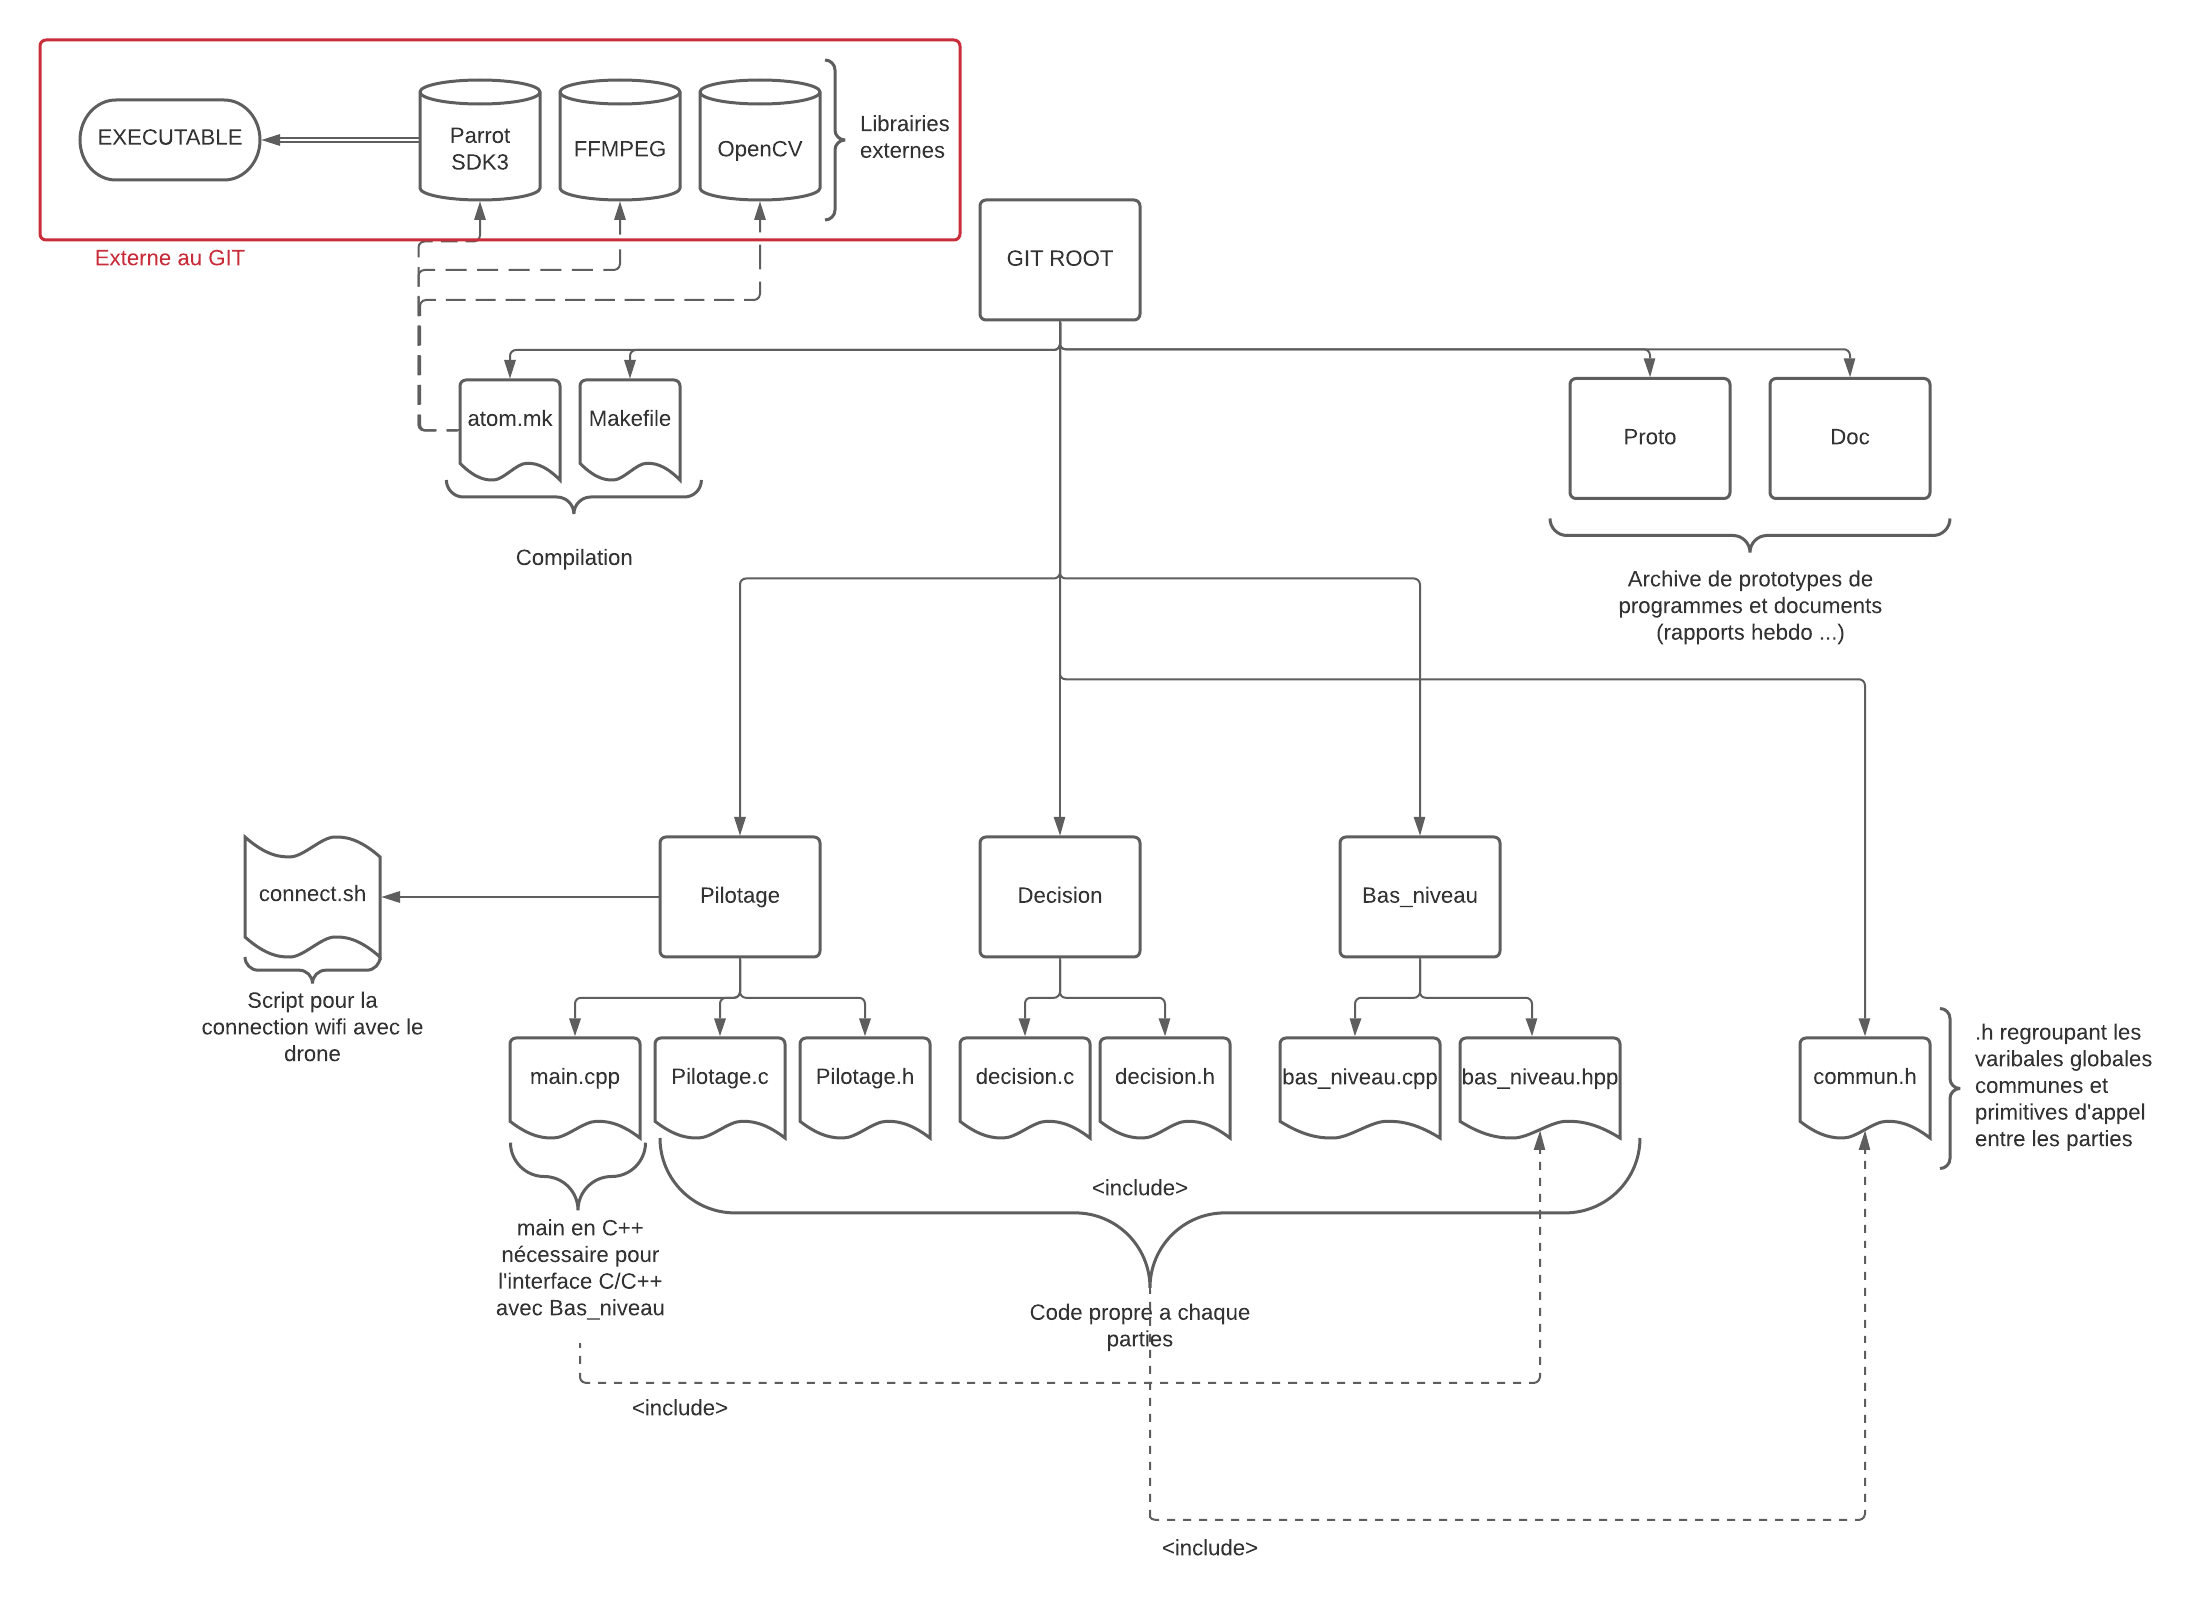
\includegraphics[height=12cm]{Architecture projet (1).png}
\caption{Architecture de la forge}
\label{fig:archi}
\end{figure}
\subsection{Intégration\label{inte}}
\paragraph*{Compilation:\label{compi}}
Pour la compilation et l'exécution de programmes, le Parrot SDK3\cite{SDK} utilise un système de build appelé Alchemy\cite{alchemy}, il permet de simplifier la gestion des makefiles, seul un makefile local "atom.mk" (cf. Figure \ref{fig:archi}) est nécessaire par application et permet de gérer toutes les dépendances. Outre l'API fourni par parrot (Parrot SDK3\cite{SDK}), nous avons utilisé ffmpeg\cite{FFMPEG} et OpenCV\cite{OpenCV}, le fichier "atom.mk" nous a donc permis de d'intégrer correctement ces différentes librairies et le code C et C++ de chaque partie simplement.

\paragraph*{Rôle du commun.h:}
Pour gérer les conventions sur les interfaces entre les parties, les variables globales et primitives communes, nous avons tout regroupé dans un fichier commun.h.\\
\begin{figure}[H]
\centering
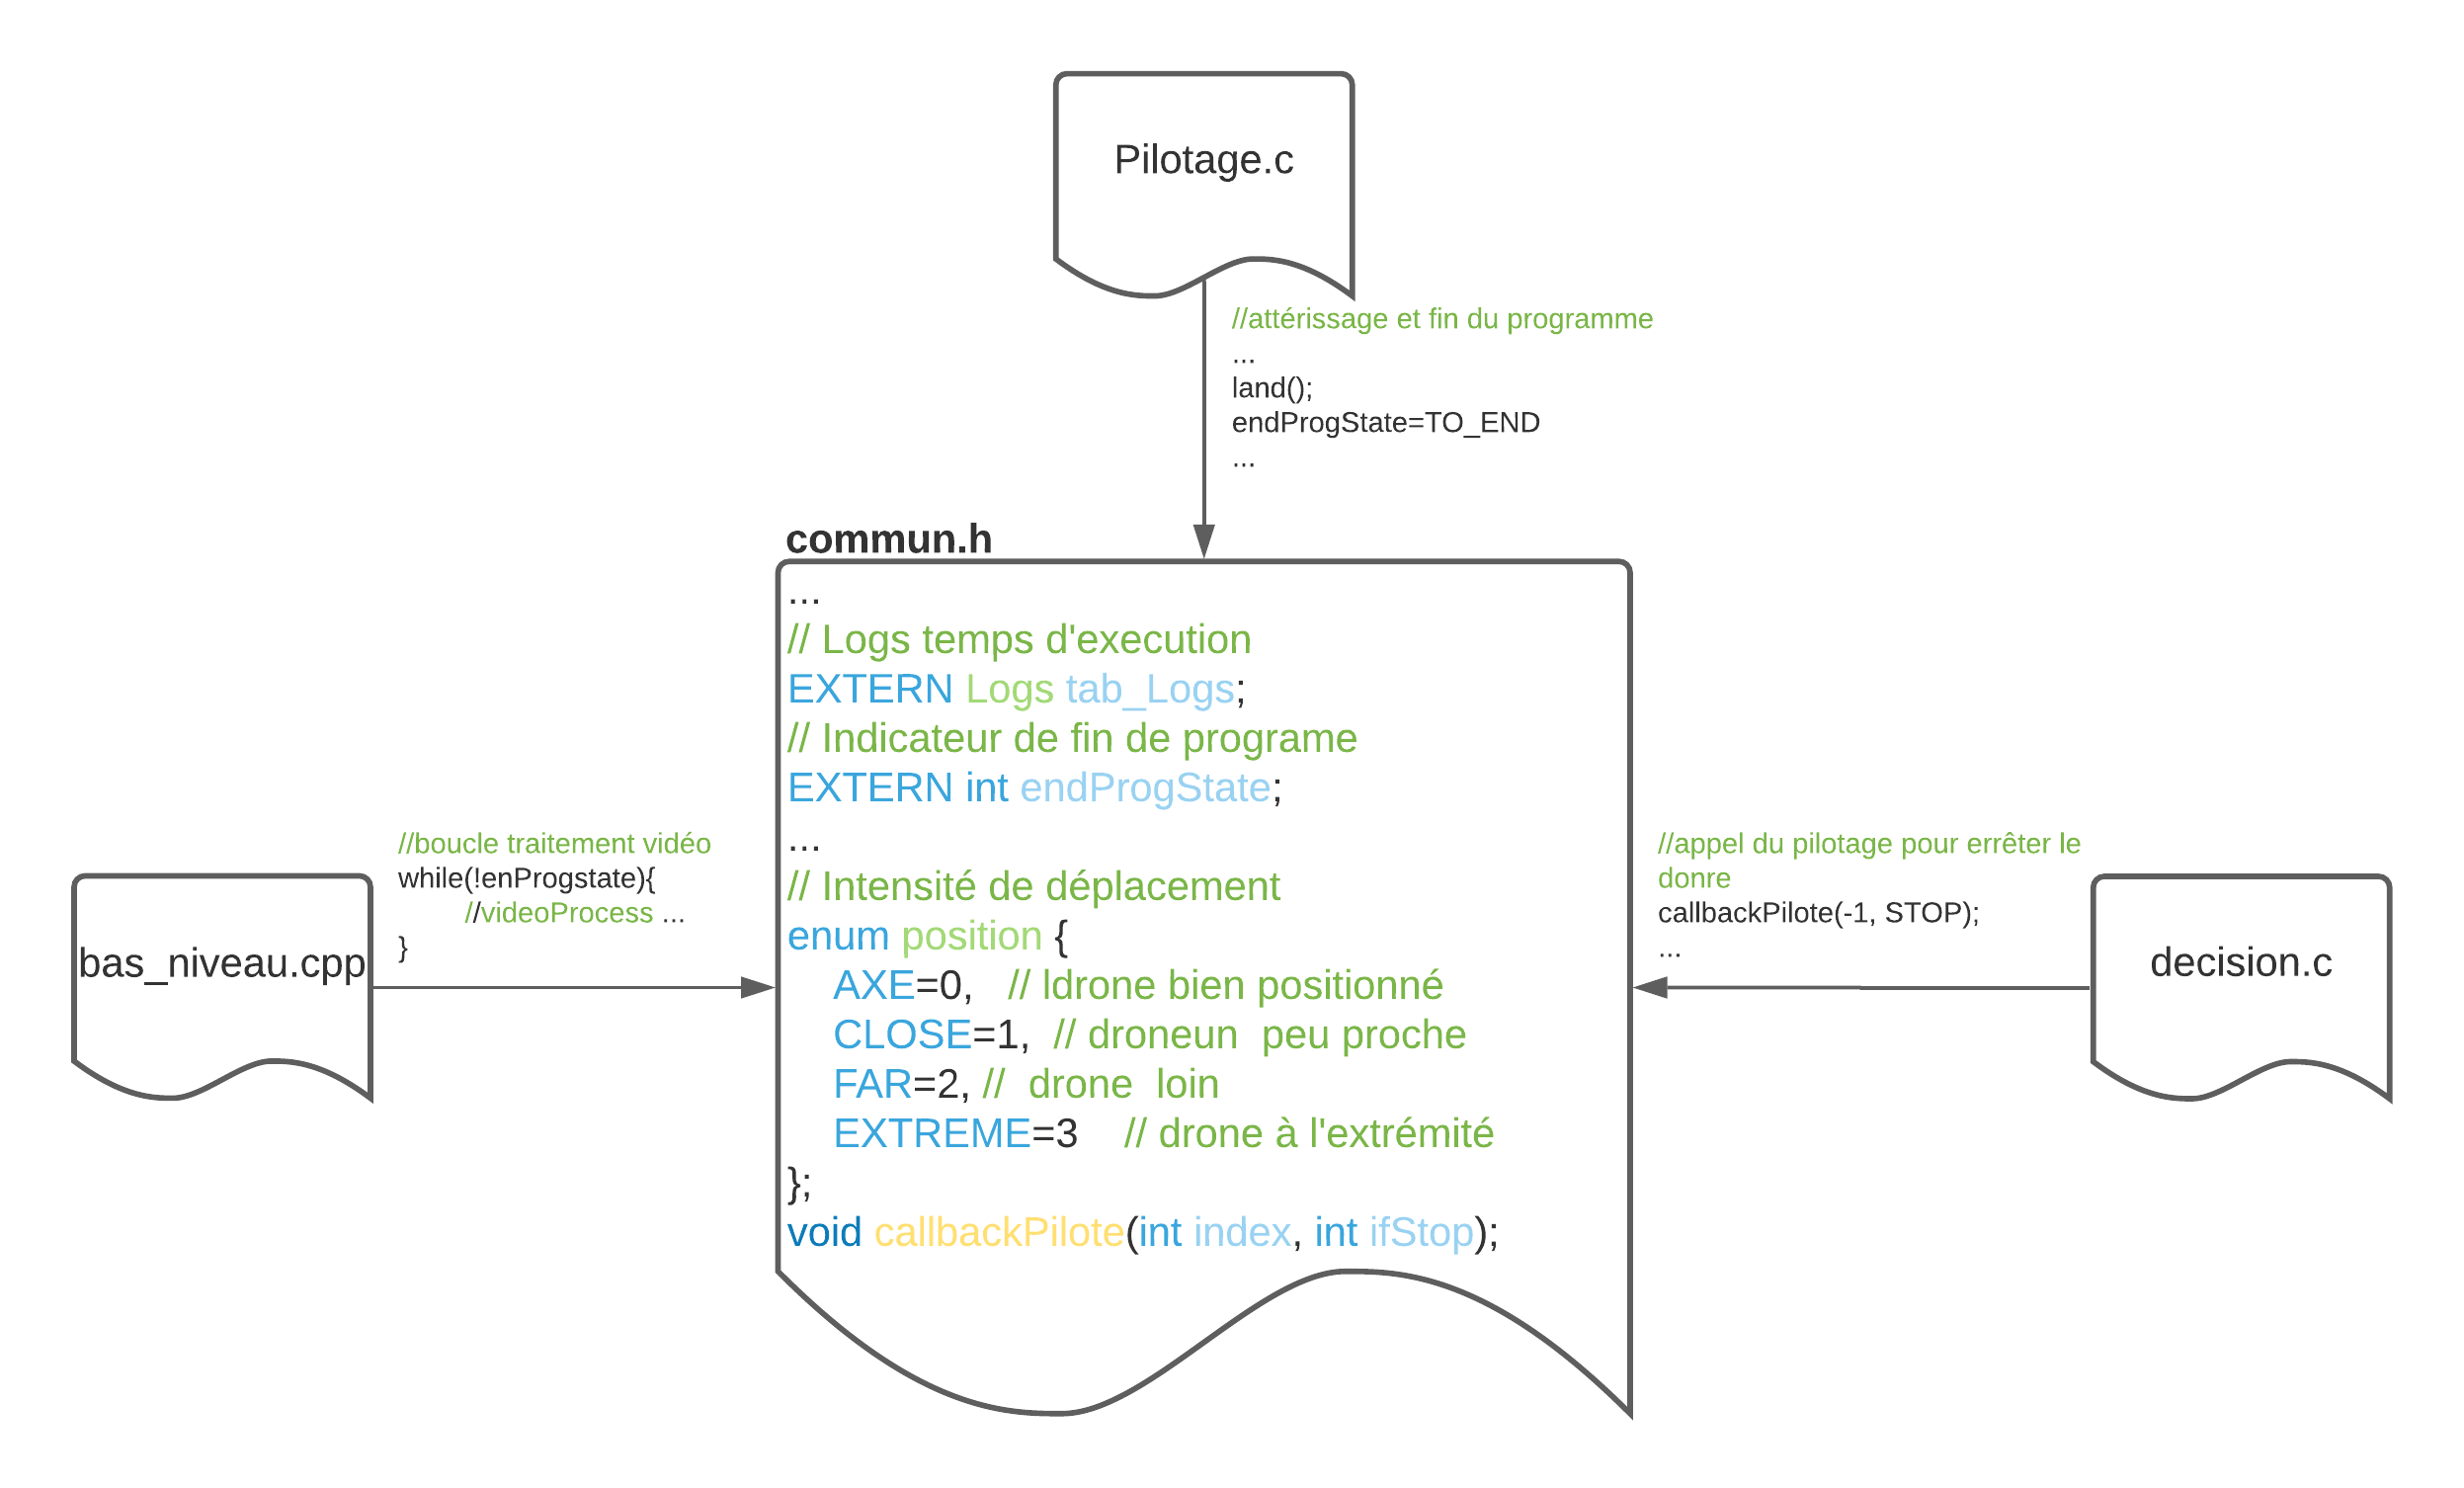
\includegraphics[height=6cm]{ExCommun.png}
\caption{Exemple utilisation commun.h}
\label{fig:commun}
\end{figure}
On va y retrouver par exemple les tableaux des logs du programme pour les calculs de temps d'exécution, des variables globales permettant le bon démarrage et la bonne synchronisation et terminaison des différents fils d'exécutions.\\
On y retrouve aussi principalement les conventions de l'interface Haut-niveau/Pilotage, comme des \#define et type énuméré représentant des directions (Gauche, droite, haut...), et intensités de mouvement (Loin, proche, centré).
\paragraph*{Interface C/C++ :}
Le Parrot SDK3\cite{SDK} est disponible en Java, C et Objective C, mais étant majoritairement écrit en C et sachant que de nombreux outils ont déjà été développés avec le SDK pour le Bebop 1 et 2 en C, le projet est principalement écrit dans ce langage.\\
Cependant, l'utilisation d'OpenCV oblige la partie imagerie Bas-niveau (cf. Section \ref{bas}) de développer en C++. Étant donné que la partie pilotage (C) doit fournir le flux vidéo à la partie Bas-niveau (C++), nous avons dû gérer cette interface. Pour cela nous utilisons un main en C++ (cf. Figure \ref{fig:archi}) qui inclut la primitive de traitement du flux de Bas-niveau(C++) et qui passe un pointeur sur fonction à la partie pilotage (C), nous avons bien sûr respecté les conventions d'appel C dans du C++. De cette manière, nous évitons l'appel direct de C++ dans du C, qui est bien plus complexe que de l'appel de C dans du C++.

\section{Pilotage\label{pilotage}}
\subsection{Objectifs}
Les principaux objectifs de cette partie sont les suivant.
\paragraph*{Liaison avec le drone :}
Il faut établir une connexion wifi stable avec le drone, lui envoyer des instructions et récupérer son flux vidéo pour le fournir a la partie Bas-niveau (cf. Section \ref{bas}).

\begin{figure}[H]
\centering
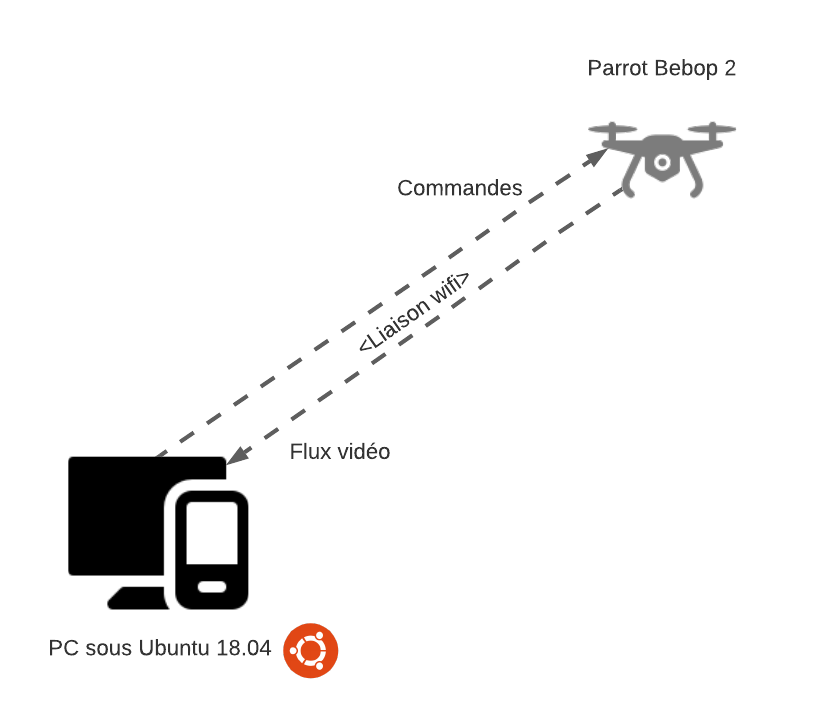
\includegraphics[height=7cm]{PCdrone.png}
\caption{Liaison PC/Drone}
\label{fig:PCdrone}
\end{figure}

\paragraph*{Pilotage du drone :}
Correctement envoyer les commandes au drone, définir les vitesses max, l'importance de l'inertie...
Il faut corréler les décisions de déplacement (cf. Section \ref{haut}) avec l'amplitude et le type de commandes (impulsions, commande longue...) à envoyer au drone.
\paragraph*{Protection du drone :}
Il faut implémenter des mécanismes de protection du drone, dans plusieurs cas d'erreurs : latence importante, perte de contrôle, gérer les signaux, exceptions ...
\subsection{Communication avec le drone}
\paragraph*{Parrot SDK3 :}
3 bibliothèques sont principalement utilisé pour communiquer avec le drone: 
\begin{itemize}
    \item libARDiscovery: trouver et établir la connexion avec le drone
    \item libARController: Contrôler le déplacement du drone
    \item libARSteam2: Récupérer et traiter le flux h264 depuis le drone
\end{itemize}

\paragraph*{Connexion au WiFi :}
Avant que libARDiscovery cherche le drone, il faut d'abord se connecter au WiFi émit par le drone, ceci est fait avant le démarrage du programme, avec le script connect.sh (cf. Figure \ref{fig:archi}).
\paragraph*{Contrôle du drone :}
Une fois le PC connecté en wifi et le drone découvert part le programme grâce à la primitive discoverDevice() (cf. Code source \cite{git}), le drone va être représenté par un objet de type ARCONTROLLER\_Device\_t  de la bibliothèque libARController ,nommé deviceController, la primitive controlDevice() (cf. Code source \cite{git}) permet d'initialiser cette variable. C'est à travers cette variable globale que toutes les instructions seront passées au drone.

\paragraph*{Récupération du flux :}
Le flux h264 est passé dans le fichier arsdk\_fifo dans le répertoire temporaire du système. En créant un pthread (cf. 2.1), nous passons ce fichier à la partie Bas\_niveau(cf\ref{bas}), qui le lit avec VideoCapture d'OpenCV\cite{OpenCV} et traite chaque image.

%Ainsi, l'affichage par mplayer et le traitemnet par ffmpeg ont été précédemment réalisés avec execlp dans un autre processus.

\subsection{Commandes}
\paragraph*{Presentation des commandes :}
Déplacement\\~\\
\begin{minipage}{.5\linewidth}
\begin{itemize}
    \item Roll:Translation(Y) Gauche/Droite 
    \item Pitch:Translation(X) Avant/Arrière 
    \item Yaw:Rotation(Z) Gauche/Droite 
    \item Gaz:Translation(Z) Haut/Bas 
\end{itemize}
\end{minipage}
\hfill
\begin{minipage}{.5\linewidth}
\centering
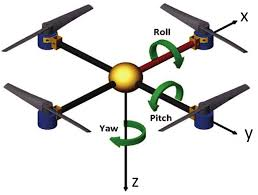
\includegraphics[width=.5\linewidth]{index.jpeg}
\end{minipage}

\subsubsection{Fonctionnement des commandes}
%\paragraph{Fonctionnement des commandes}
Une commande de déplacement envoyé au drone dépend de deux variables :
\begin{itemize}
    \item \textbf{L'intensité}: L'intensité est représenté en \% d'angle max (°) pour le Pitch/Roll et Yaw et \% de vitesse max (m/s) pour le Gaz (Haut/Bas). Comme on peux l'observer sur la Figure \ref{fig:prcangle} le \% d'angle max est défini par l'inclinaison du drone, donc l'angle par rapport à l'horizon. Il est exprimé en fonction du \% de l'angle maximal d'inclinaison (segment rouge).
    \begin{figure}[H]
    \centering
    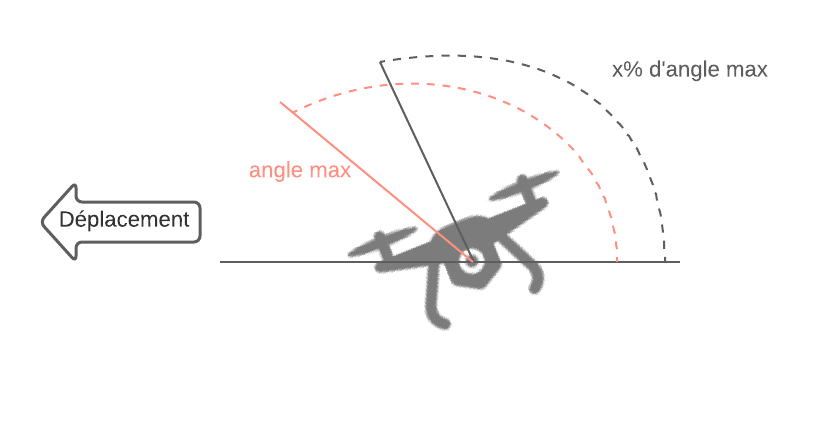
\includegraphics[height=5cm]{PrcAngle.png}
    \caption{Exemple \% Angle Max pour le Roll}
    \label{fig:prcangle}
    \end{figure}
    \item \textbf{Le temps}: Lorsqu'une commande est envoyée au drone, celle-ci est réalisée jusqu'à ce que la commande stop() (cf. Code source\cite{git}) soit envoyée, arrêtant tout déplacement du drone. De cette manière la distance déplacement du drone dépend directement de la durée de la commande. On verra dans la partie Gestion des cas d'erreurs (cf. Section \ref{err}) qu'une durée de commande imprévue (bugs dans le programme...) peux s'avérer dangereuse pour le drone. 
\end{itemize}
\subsubsection{Boucle événementielle et déplacements par impulsions}
%\paragraph*{Boucle événementielle et déplacements par impulsions:}
Comme on a pu le voir dans le principe de fonctionnement du projet(cf Section .\ref{principe}),le système d'envoi de commande est régi par une boucle événementielle (cf Figure \ref{fig:imp}).
\begin{figure}[H]
\centering
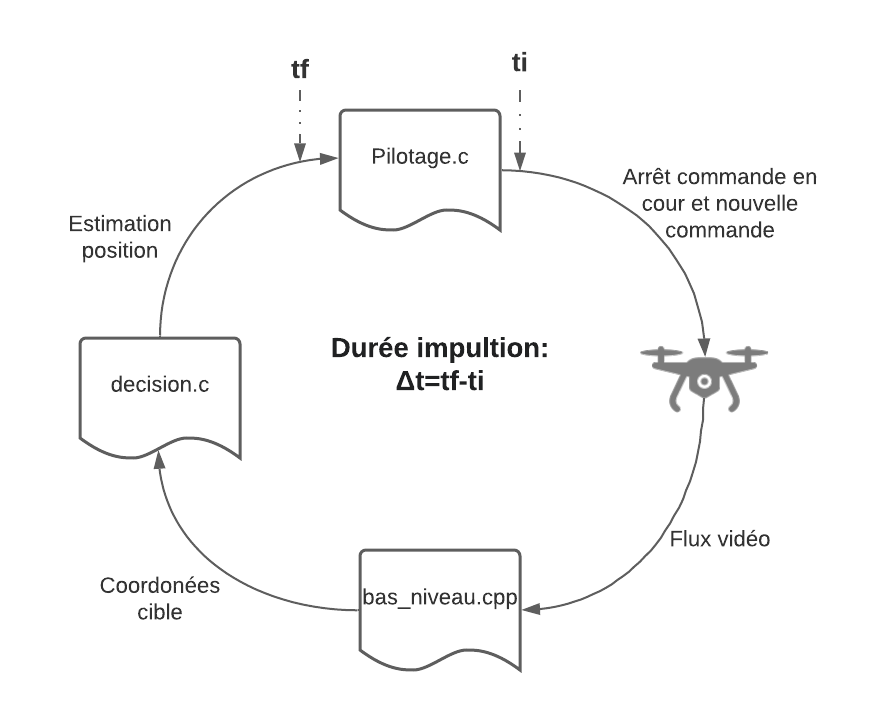
\includegraphics[height=6cm]{DureeImp.png}
\caption{Durée impulsion}
\label{fig:imp}
\end{figure}
Une commande est donc envoyée, un tour de boucle est réalisé (traitement Bas-niveau et Haut-niveau) et au nouveau tour de boucle la commande précédente est stoppée. C'est donc \textbf{la durée de la boucle qui définira la durée d'une commande}, ce principe de fonctionnement nous oblige donc a fonctionné avec des "impulsions". On a dû donc tester le comportement du drone avec ce genre de déplacement (cf. Section \ref{proex}). Le drone réagit très bien aux courtes impulsions, de cette manière, on est aussi beaucoup plus précis dans nos déplacements, d'un autre côté le temps d'exécution d'une boucle et sa variation vont jouer un rôle important dans les déplacements du drone et donc dans des déplacements inattendu (cf. Section \ref{err}).
Pour définir \textbf{l'intensité des déplacements}, nous avons en accord avec la partie Haut\_niveau (cf. Section \ref{haut}) défini trois niveaux d'impulsions (FORT,MOYEN,FAIBLE) correspondant à trois distances à la cible (TRES LOIN,LOIN,PROCHE), ces constantes on été définies lors de séances de calibration (cf. Section \ref{proex}).

\subsection{Gestion des cas d'erreurs\label{err}}
Plusieurs protocoles ont été mis en place afin d'assurer la robustesse du programme et la sécurité du drone.
\paragraph*{Terminaison du programme:}
A cause de la multiplicité des threads, des éventuelles erreurs fatales ou bien d'un atterrissage, il est nécessaire de terminer le programme proprement.\\
La fonction endProg() est alors appelée : 
\begin{itemize}
    \item Arrêter et faire atterrir le drone
    \item Supprimer le deviceController
    \item Terminer le flux et fermer le ficher du flux
\end{itemize}
L'état de la terminaison du programme est décrit par la variable endProgState (cf. Code source\cite{git}).Afin d'éviter l'appel redondant de endProg() (threads multiples), elle ne sera appelée qu'à la condition ou endProgState n'est pas à ENDING. Au début de l'exécution endProgState est à RUNNING,quand le programme doit se terminer la variable passe a TO\_END (il faut appeler endProg()), enfin à l'appel de endProg() la valeur de endProgState passe à ENDING pour bloquer les autres tentatives d'appel.

\paragraph*{Watchdog :}
12 fois par seconde, la fonction callbackPilote est appelée pour envoyer la nouvelle commande au drone, cela garantit le déplacement correct du drone. Donc, pour le fonctionnement du programme et la sécurité du drone, il est crucial d'assurer que la fréquence d'appel de callbackPilote soit constante. De là, un mécanisme de Watchdog a été créé.

Dès l'appel du premier callbackPilote, le Watchdog se réveille au début de chaque cycle (défini comme CYCLE), il compare le décalage entre le compteur du temps mis à jour par le callbackPilote le plus récent, et le temps réel. Si ce décalage est supérieur que la limite prédéfinit (TIMEOUT), le Watchdog appellera la fonction endProg pour faire atterrir le drone et terminer le programme, terminant l'état du vol aveugle.

\paragraph*{Récupération de Signaux :}
La terminaison inattendue non traitée peut être très dangereuse, car elle interrompt le programme sans arrêter le drone. Pour cette raison, tous les signaux envoyés par le système qui peuvent interrompre l'exécution seront récupérés et amenés à la fonction catchSig, qui affiche le numéro du signal récupéré et qui appelle endProg pour terminer le programme correctement.

Grâce à ce mécanisme, il est aussi possible d'envoyer un SIGINT (Control-C) à tout moment pour terminer le programme et faire atterrir le drone. Cela permet l'interruption manuelle en cas d'urgence.

\paragraph*{Gestion des Exceptions:}
Dans la boucle événementielle, des exceptions peuvent être levées, ces exceptions peuvent être fatale ou non-fatale. A la récupération de l'exécution, l'exception sera analysée pour décider s'il faut appeler callbackPilote pour terminer le programme ou ignorer l'exception et continuer la boucle. À la récupération de l'exécution, l'exception sera analysée pour décider s'il faut appeler callbackPilote pour terminer le programme ou ignorer l'exception et continuer la boucle. 

\subsection{Synthèse des mécanismes de pilotage\label{synpilote}}
Voici un schéma plus précis basé sur celui de la Figure \ref{fig:fctprecis} synthétisant les mécanismes permettant de piloter et contrôler le système. La syntaxe utilisée est exactement celle du projet (cf. Code source\cite{git}). On y retrouve les trois threads, le principal, qui s'occupe d'attraper les signaux (rouge), le watchodg (bleu) et la boucle événementielle (vert) qui est lancée à travers une boucle de la fonction vidéo\_reader\_process() (traitement de chaque image et appel de l'analyse de haut-niveau).\\
On y retrouve aussi le main\_Pilotage qui prend en paramètre functionPtr, qui comme expliquer dans la section Intégration (cf. Section \ref{inte}) permet de facilité l'interface C/C++ avec l'appel de vidéo\_reader\_process() depuis le main\_Pilotage().
\begin{figure}[H]
\centering
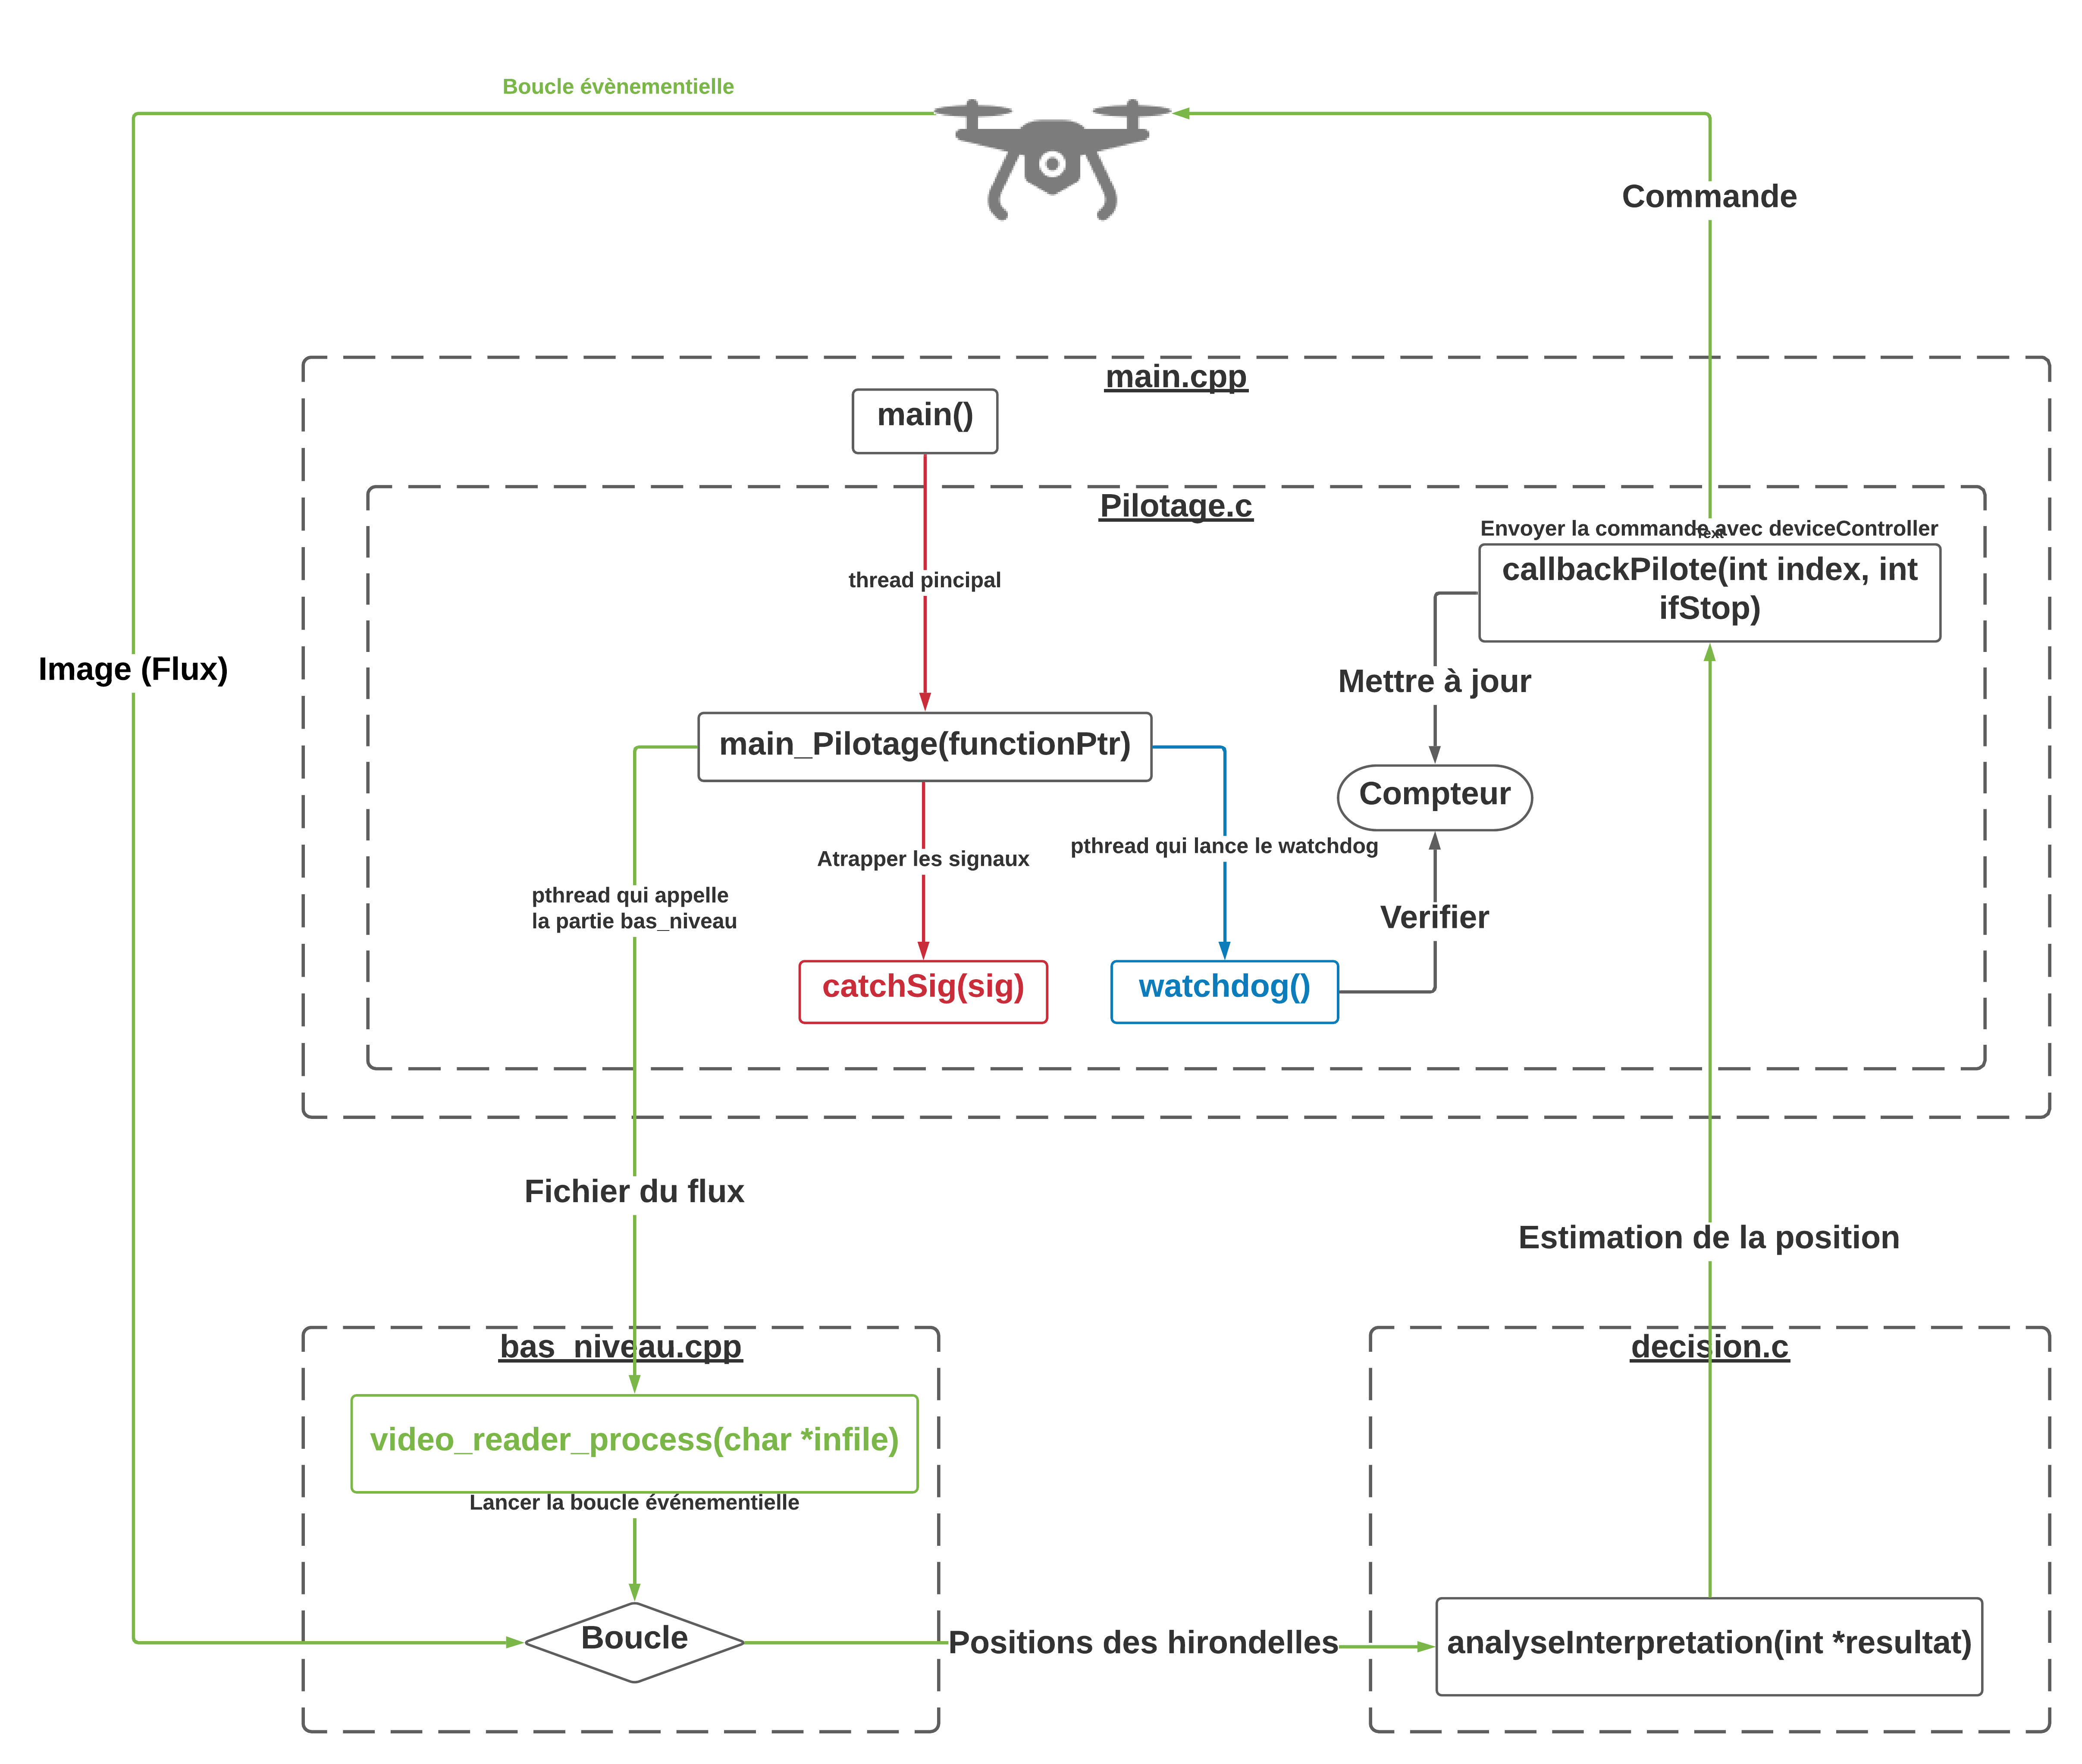
\includegraphics[width=16cm]{Fonctionnement.png}
\caption{Fonctionnement des mécanismes}
\label{fig:fctprecis}
\end{figure}

\subsection{Protocole expérimental\label{proex}}
Pour pouvoir tester nos programmes avant de réaliser des tests sur le drone physique (par sécurité), nous avons utilisé le simulateur développé par Parrot.
\subsubsection{Tests sur simulateur}
%\paragraph*{Tests sur simulateur:}
Parrot-Sphinx\cite{sphinx} est un outil de simulation initialement pensé pour couvrir les besoins des ingénieurs Parrot. Le simulateur est de très bonne qualité et prend en compte de manière très précise les moindres variation d'impulsion, l'inertie ...
\begin{figure}[H]
\centering
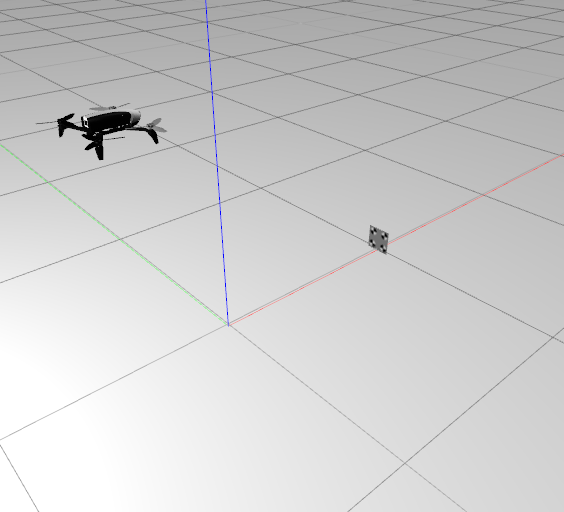
\includegraphics[height=5cm]{Sphinx.png}
\caption{Drone et cible dans le simulateur}
\label{fig:sphinx}
\end{figure}
La manipulation du simulateur (connexion au drone...) est en tous points similaire au drone physique, le simulateur tourne sur une deuxième machine (sous ubuntu 18.04) à laquelle on se connecte. On a modélisé une cible pour ensuite l'intégrer a l'environnement du simulateur (cf. Figure \ref{fig:sphinx}), de cette manière, tous les prototypes de programme jusqu'à la version finale du projet ont pu être testés sur Sphinx\cite{sphinx} avant les tests sur le drone physique.\\

\subsubsection{Limites du simulateur}
%\paragraph*{Limites du simulateur:}
Bien évidemment, le simulateur a ses limites, la prise en compte de l'inertie est limité, d'autant plus quand les mouvements sont composés (nous avons d'ailleurs du changer notre protocole de déplacement pour prendre en compte cette différence). L'environnement du simulateur est "parfait", bonne lumière, pas d'objet qui interfère avec la cible. Au niveau de la liaison wifi, la liaison avec la machine qui supporte le simulateur est le plus souvent stable alors qu'avec le drone, celui est en mouvement, il est donc arrivé de perdre la connexion avec le drone lors de séance de test avec le drone physique.
On a pu grâce à une séance de calibrage avec le drone physique, étudier l'évolution des déplacements du drone en fonction du nombre d'impulsions envoyé, et comparé les résultats obtenus entre le simulateur et le test réel (cf. Figure \ref{fig:diffsimu}) 

\begin{figure}[H]
\centering
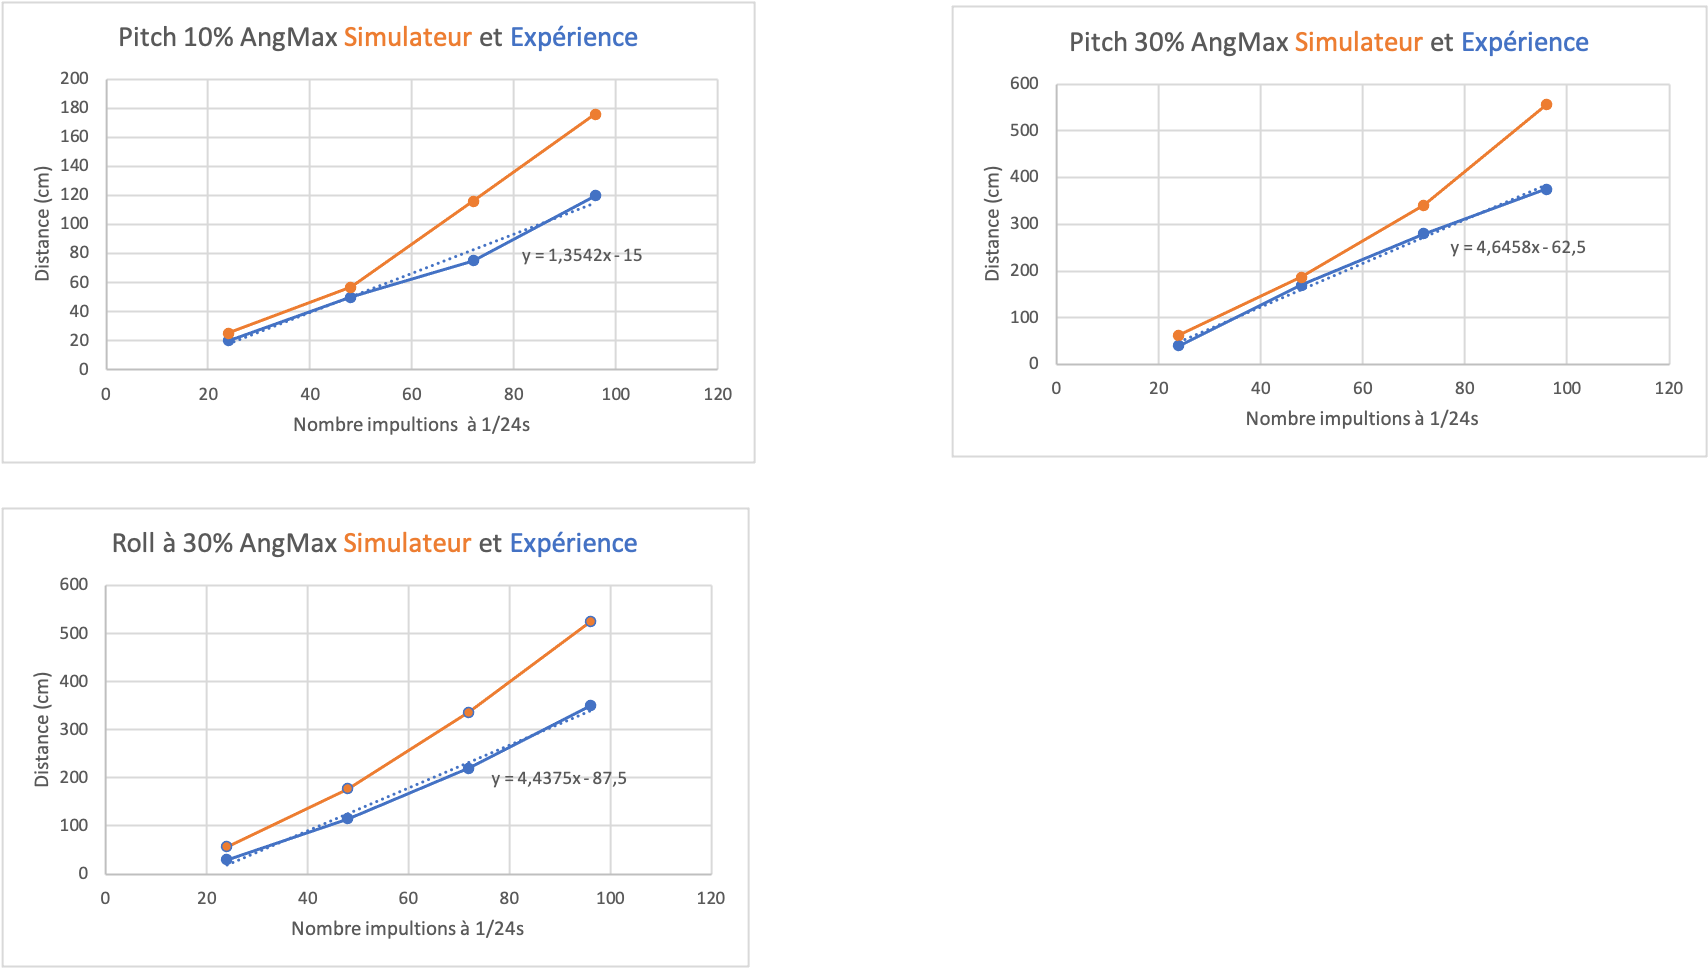
\includegraphics[height=9cm]{DiffSimu.png}
\caption{Différence entre simulateur et test physique}
\label{fig:diffsimu}
\end{figure}

On observe que systématiquement à nombre d'impulsions égale, les déplacements sur le simulateur sont plus important, cela est sûrement du au fait que l'état des moteurs est "parfait" sur le simulateur, même chose pour la batterie, le simulateur ne prend pas en compte l'usure des composants ,on a donc des différences de puissance. On a pris en compte ces différences lors de nos tests. Nous avons tracé des droites de tendance (pointillés) pour les courbes de tests physiques (bleu), elle nous on permis d'avoir une idée des distances qu'allait parcourir le drone et donc de fixé les constantes d'intensité de déplacement. 

\section{Imagerie de bas niveau\label{bas}}


\subsection{Objectifs}
L'objectif de cette partie est d'analyser le flux vidéo capturé par la caméra du drone, et réaliser les deux premières étapes du traitement d'image : \\         
\textbf{Prétraitement : }opérations de
manipulation de l'image pour améliorer la
qualité, car il est impératif d'extraire la bonne information à bas niveau.\\
\textbf{Analyse : }suite d'opérations pour l'extraction
d'informations contenues dans une image. Dans ce projet, l'information qui nous intéresse est la présence ou non de la cible; et dans le cas favorable, sa position sur l'image.


\subsection{Entrée et sortie de la partie }
\label{section:Workflow}
 \begin{figure}[H]
\centering
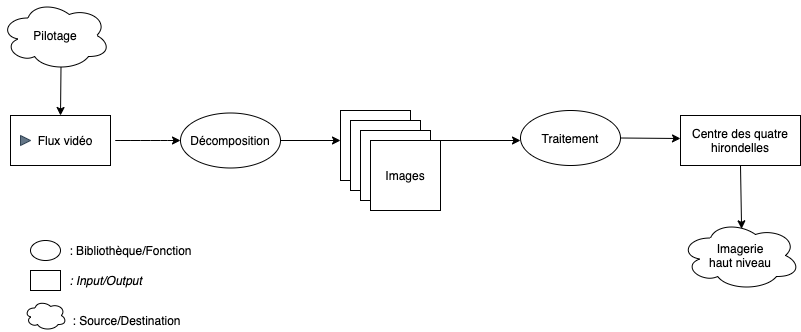
\includegraphics[height=6cm]{workflowG.png}
\caption{Schéma représentatif des différentes entrées sorties de la partie imagerie bas niveau. }
\label{fig:WorkflowG}
\end{figure}


La partie relative à l'imagerie bas niveau est divisée en deux parties principales (cf. Figure \ref{fig:WorkflowG}).\\ L'étape 1 concerne le traitement du flux vidéo récupéré de la partie pilotage. Il est décomposé pour en extraire des images. \\Ces images sont traitées au cours de la deuxième étape qui consiste à leur appliquer des algorithmes de traitement d'images.\\ L'objectif est de récupérer les coordonnées des quatre hirondelles de la mire.\\
La partie imagerie haut niveau aura en entrée ces coordonnées.



\subsection{Traitement d'image}
\label{section:Traitement}

 \begin{figure}[H]
\centering
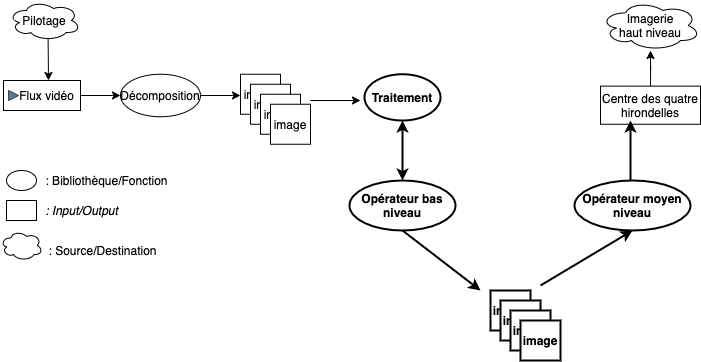
\includegraphics[height=7cm]{workflowI.png}
\caption{Schéma représentatif des différentes entrées sorties de la partie imagerie bas niveau en zoomant sur la partie traitement. }
\label{fig:WorkflowI}
\end{figure}

Ce schéma met en avant la deuxième étape du traitement du flux. Elle consiste à analyser les images.
Nous pouvons en distinguer deux étapes successives : opérateur bas niveau et opérateur moyen niveau qui sont détaillés ci-dessous.

\subsubsection{Opérateur bas niveau }
Cette partie concerne le traitement bas niveau sur les images reçues afin d'améliorer leur qualité.\\
Les images reçues sont en couleur. La première étape consiste à les transformer en images à niveau de gris.

\paragraph*{\textbf{Pourquoi ce traitement ?}} une image en couleur est constituée de trois couches: une couche rouge (R), une couche verte (V), une couche bleue (B). Soit Nx le nombre de colonnes de l'image et Ny le nombre de lignes.\\ Le nombre de pixels total est $N=Nx * Ny$. Chaque couche est une matrice comportant Ny lignes et Nx colonnes. Le plus souvent, cette matrice contient des entiers codés sur 8 bits (les valeurs vont de 0 à 255). Pour l'image en couleur complète, il y a donc 24 bits par pixels, à multiplier par le nombre de pixels pour obtenir l'occupation totale en mémoire.\\
Cela est évidemment très coûteux en mémoire. La transformation en image à niveau de gris permet de minimiser la taille de chaque image.\\ Une autre raison est que la mire est composée d'un motif de couleur noire et blanche. Les valeurs des couches rouge, verte et bleue ne sont pas nécessaires pour détecter la mire.   




\subsubsection{Opérateur moyen niveau }
Le but de cette partie est de détecter et retourner les coordonnées des centres des 4 hirondelles de la mire.\\
Afin de détecter les points d'intérêts, l'approche utilisé est à base de modèles : ces points sont identifiés dans l’image par mise en correspondance de leur intensité avec un modèle théorique des intensités, vu que la couleur et la forme de la mire sont déjà connues.\\
Ce traitement est basé un motif qui consiste à obtenir un résultat proche de 0 en sommant les pixels voisins de chaque pixel de la manière présentée ci-dessous :\\

 \begin{figure}[H]
\centering
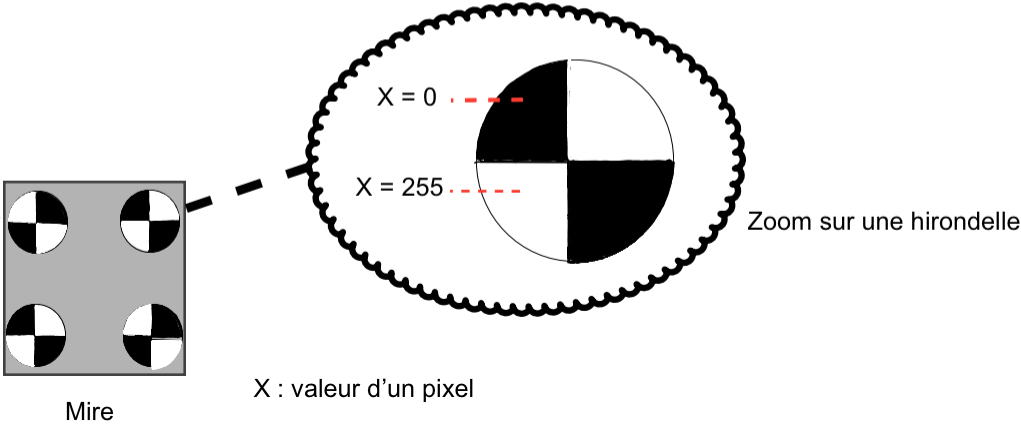
\includegraphics[height=4cm]{B_Shema1.jpg}
\caption{Schéma illustrant les valeurs des pixels de la mire dans un modèle théorique. }
\label{fig:calcul}
\end{figure}


Soient $\{a1 , a2 , a3,...,ar\}$ l'ensemble des pixels qui constituent le voisinage du point a traiter. Soit N le voisinage choisi ( par exemple N= 3x3 , 2x2 ...etc)\\


Soit X la somme des pixels : $X = a1 + a2+ a3 +...+ar $
Alors, pour les cibles d'en haut, On calcule : $S = S1 + S2 +S3 + S4$ avec :\\
 S1 = X \\
S2 = $(255*N) - X $ \\
S3 = X \\
S4 = $(255*N) - X $ \\

Identiquement, pour les cibles d'en bas : 
$S = S1 + S2 +S3 + S4$ avec : \\
S1 = $(255*N) - X $ \\
S2 = X \\
S3 = $(255*N) - X $ \\
S4 = X \\
 
Dans un résultat théorique, la somme est nulle pour les centres des hirondelles. Néanmoins, ce n'est pas le cas en pratique. Les points à retourner  sont les points avec la somme minimum.

\begin{figure}[H]
\centering
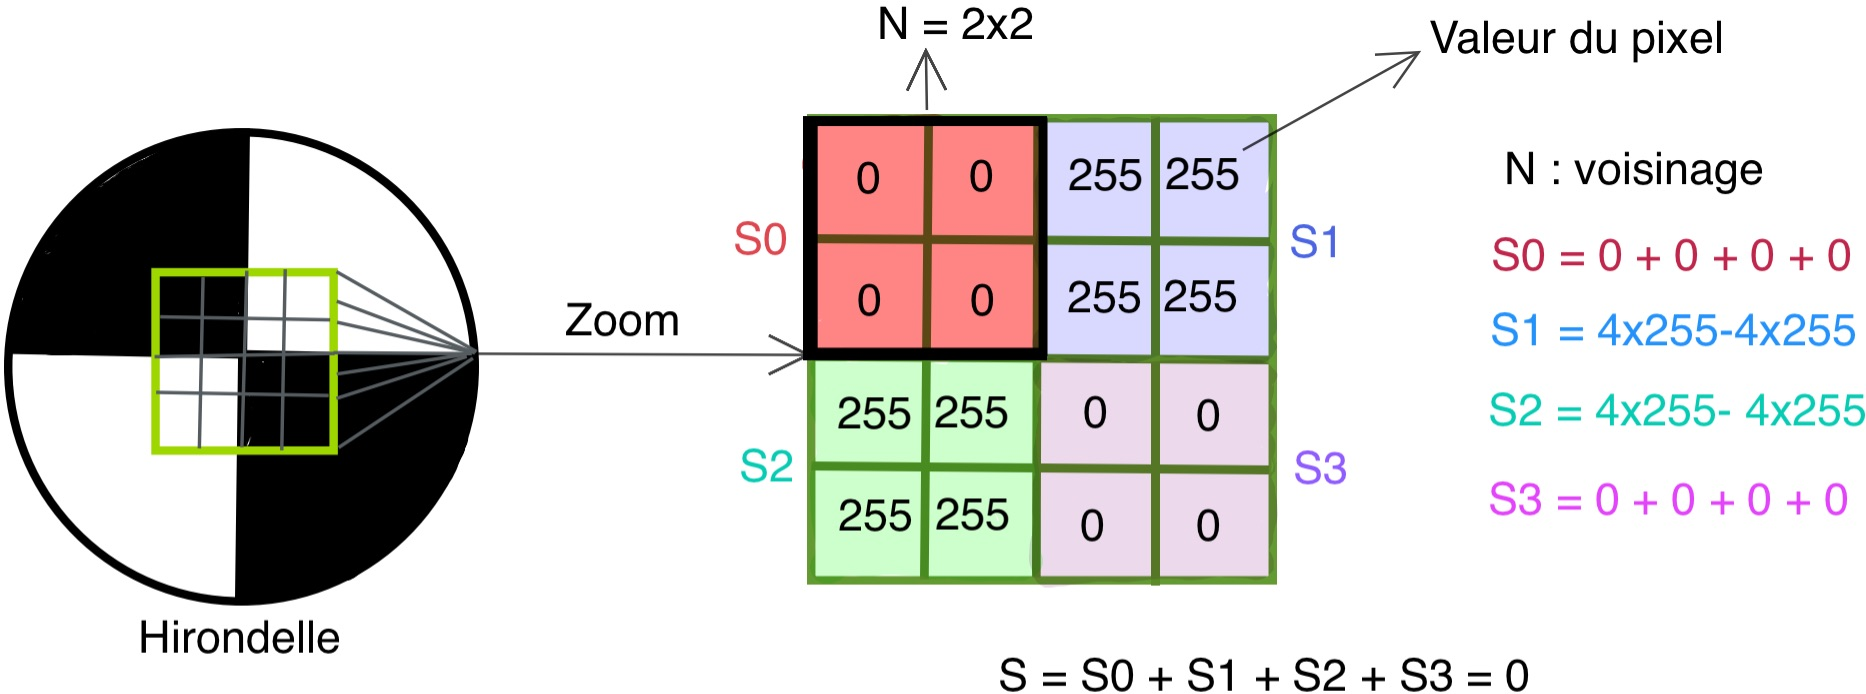
\includegraphics[height=5cm]{B_theorique.png}
\caption{Schéma représentatif du résultat du calcul pour un modèle théorique parfait. }
\label{fig:calcul_theorique}
\end{figure}

\subsection{Détection }
Au cours de ce traitement, nous avons ajouté la contrainte d'espacement entre deux points, dans le sens où si deux points sont assez proches (d'une marge de pixels qui varie selon la distance entre la mire et le drone), ils sont considérés comme un seul point (appartenant à une seule hirondelle).\\ Il est donc plus judicieux de considérer d'autres points minimums de la mire pour détecter les autres hirondelles et de ne considérer qu'un point par hirondelle.\\
Pour éviter qu'une hirondelle soit détectée plusieurs fois,  un étalonnage a été réalisé sur les images selon les distances pour essayer de déterminer l'espacement minimum que deux hirondelles doivent respecter.

\subsection{Problèmes rencontrés lors de la détection}
\begin{enumerate}
        \item \textbf{Influence de l’environnement :}
nous avons appliqué l’algorithme de détection sur des vidéos prises par le drone et nous avons très vite constaté que l’environnement (luminosité et  l’arrière plan) avait un impact direct sur la détection de la mire. En effet, s’il y a des motifs qui ressemblent aux hirondelles de la mire, ils peuvent être confondus et considéré comme mire (cf. Figure~\ref{fig:environnement}).\\
\begin{figure}[H]
    \centering
    \subfloat[cage de handball détectée]{{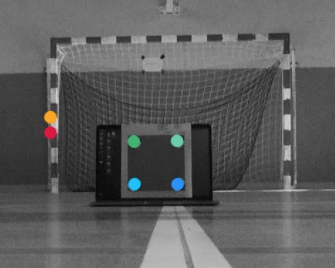
\includegraphics[width=5cm]{B_handball.png} }}
    \qquad
    \subfloat[coin de la feuille et cage de handball détectés
    ]{{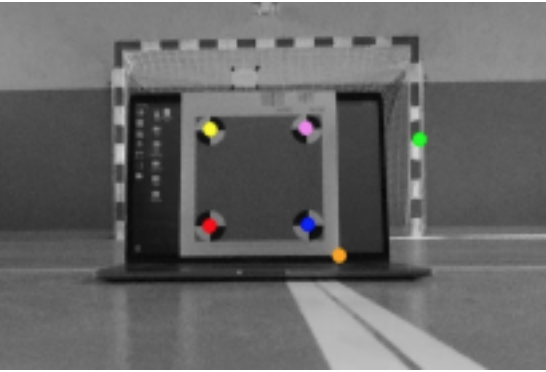
\includegraphics[width=6cm]{B_feuille.png} }}
    \caption{Influence de l'environnement sur la détection des points d'intérêt.}
    \label{fig:environnement}
\end{figure}

Cette figure représente une image d'une vidéo prise dans le centre sportif Jean Talbot. La transformation en image à niveau de gris fait que la cage de handball qui était initialement en rouge et blanc, est représentée à présent en gris foncé et blanc. \\ 
L'alteration de couleur gris-blanc ressemble au motif des hirondelles de la mire. Elles sont donc détectées par l'algorithme. 



\item \textbf{Distance de détection : } la détection des hirondelles devient plus difficile en s'éloignant de la mire, ce qui est logique.\\ Premièrement, nous faisons varier le voisinage en l'augmentant dès lors qu'on se rapproche de la mire mais cela a un impact sur le temps de traitement et génère donc une grande latence.\\ Il est donc nécessaire de trouver une solution qui permettrait d'augmenter la portée de la détection sans pour autant influencer le temps de calcul.  

\item \textbf{Ratio des sommes : } en premier lieu, le calcul des ratios consiste à déterminer trois points de sommes minimums pour chaque ensemble d’hirondelles ( celles du haut et celles du bas). \\
Soient a, b, c les trois points minimums correspondants -par exemple aux minimums calculés avec la somme des hirondelles du bas ordonnés par ordre croissant. \\
Nous allons calculer trois ratios qui sont : c/a , c/b , b/a. Théoriquement, si la mire est présente, alors nous allons obtenir un ratio proche de 1, et deux autres avec une valeur plus grande.\\ 
Cependant, nous avons remarqué pendant les tests que le ratio calculé ne nous donne pas une réelle estimation de la présence de la mire sur l’image. 


Cela est dû au fait que l'algorithme considère que les sommes obtenues grâce aux pixels voisins à celle de l’hirondelle (à un, deux ou trois pixels près) comme l’un des minimums recherchés, de ce fait une hirondelle peut être considérée plusieurs fois comme point d’intérêt et cela est contraignant. \\

En second lieu, nous avons introduit une distanciation minimale exigée par notre algorithme afin d’éliminer le cas cité précédemment grâce a plusieurs tests d’étalonnage et en calculant la distance euclidienne minimale pour séparer deux hirondelles, les sommes obtenues après ce changement ne sont toujours pas satisfaisantes et le calcul du ratio ne nous aide toujours pas. \\
\begin{figure}[H]
    \centering
    \subfloat[Photo issue d'une vidéo prise par notre ordinateur.]{{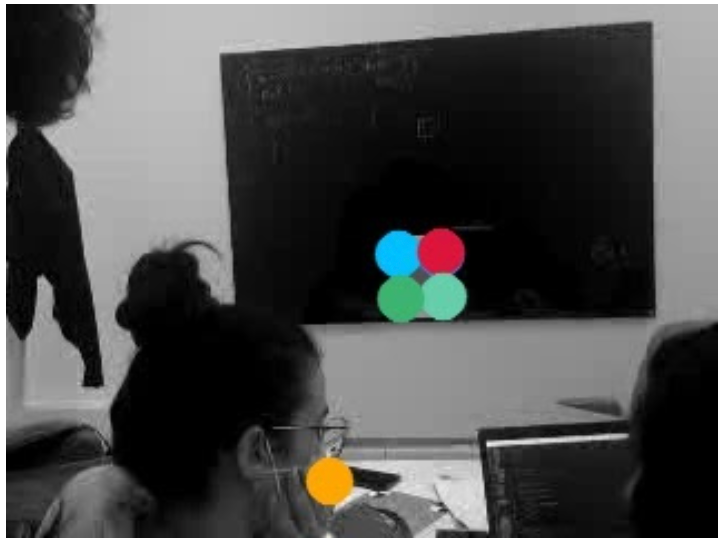
\includegraphics[width=4cm]{B_Ratio.png} }}
    \qquad
    \subfloat[Sommes obtenues
    ]{{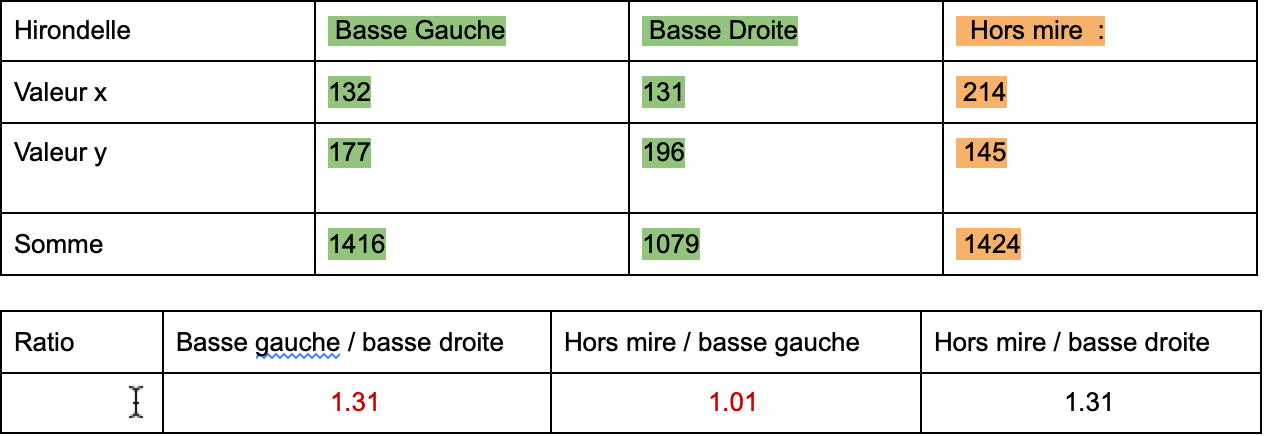
\includegraphics[width=9cm]{B_tableau_ratio.png} }}
    \caption{Résultat illustrant les valeurs du ratio}
    \label{fig:ratio}
\end{figure}

La figure ci-dessus présente un exemple de résultat de l'algorithme sur une vidéo prise par la caméra de notre ordinateur.\\
Le tableau représente les points retournés qui sont affichés dans l'image.\\ La valeur qui nous intéresse est le calcul de la somme pour les points des hirondelles du bas.\\
Nous obtenons un point hors de la mire dont la valeur de la somme obtenue est très proche de celles des points qui représentent la mire.\\

La raison pour cela est que dans certains environnements, nous obtenons des points avec des sommes proches de celles de la mire (un exemple est celle des cages de but dans le centre sportif Jean Talbot peintes en rouge et blanc: point vert (cf. Figure~\ref{fig:environnement}), ou bien le bord de la feuille de la mire que nous avons imprimée de couleur blanche: point orange (cf. Figure~\ref{fig:environnement}). \\
Dans d’autres cas cela peut être simplement le bord de la fenêtre (cf. Figure~\ref{fig:fenetre}) ou un motif sur nos vêtements. 
 \begin{figure}[H]
\centering
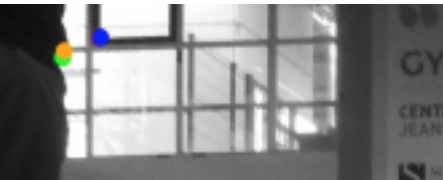
\includegraphics[height=3cm]{B_fenetre.png}
\caption{Détection de points sur la fenêtre.}
\label{fig:fenetre}
\end{figure}

En fin de compte, il est impératif de trouver d’autres stratégies pour éliminer les points qui sont en dehors de la mire.



\item \textbf{Latence : } après avoir implémenté l’algorithme de traitement d’image nous avons constaté une grande latence dû aux gros calculs matriciels, et cela a un impact direct sur les mouvements du drone si ce n’est la partie qui consomme le plus de temps.

\item \textbf{Robustesse de la détection des points : } 
même en présence de la mire, les images peuvent contenir des points minimums meilleurs que ceux de la mire, cela rend la tâche de détection plus difficile et nous devions donc implémenter des stratégies pour augmenter la robustesse de la détection en éliminant des points qui a priori ne peuvent pas représenter la mire malgré leurs sommes très basses.


\end{enumerate}


\subsection{Solutions aux problèmes }
\begin{enumerate}
\item \textbf{Choix de l'environnement :  } afin d'éviter qu'en présence de la mire des points hors la mire soient considérés comme points d'intérêt, une contrainte sur l'environnement de test doit être faite.\\ 
L'environnement de test doit être lumineux, il faut éviter les motifs qui ressemblent aux hirondelles, et éviter les fenêtres (effet contre jour).

\item \textbf{Distance de détection : } 
agrandir les hirondelles.
\begin{figure}[H]
    \centering
    \subfloat[Ancienne mire]{{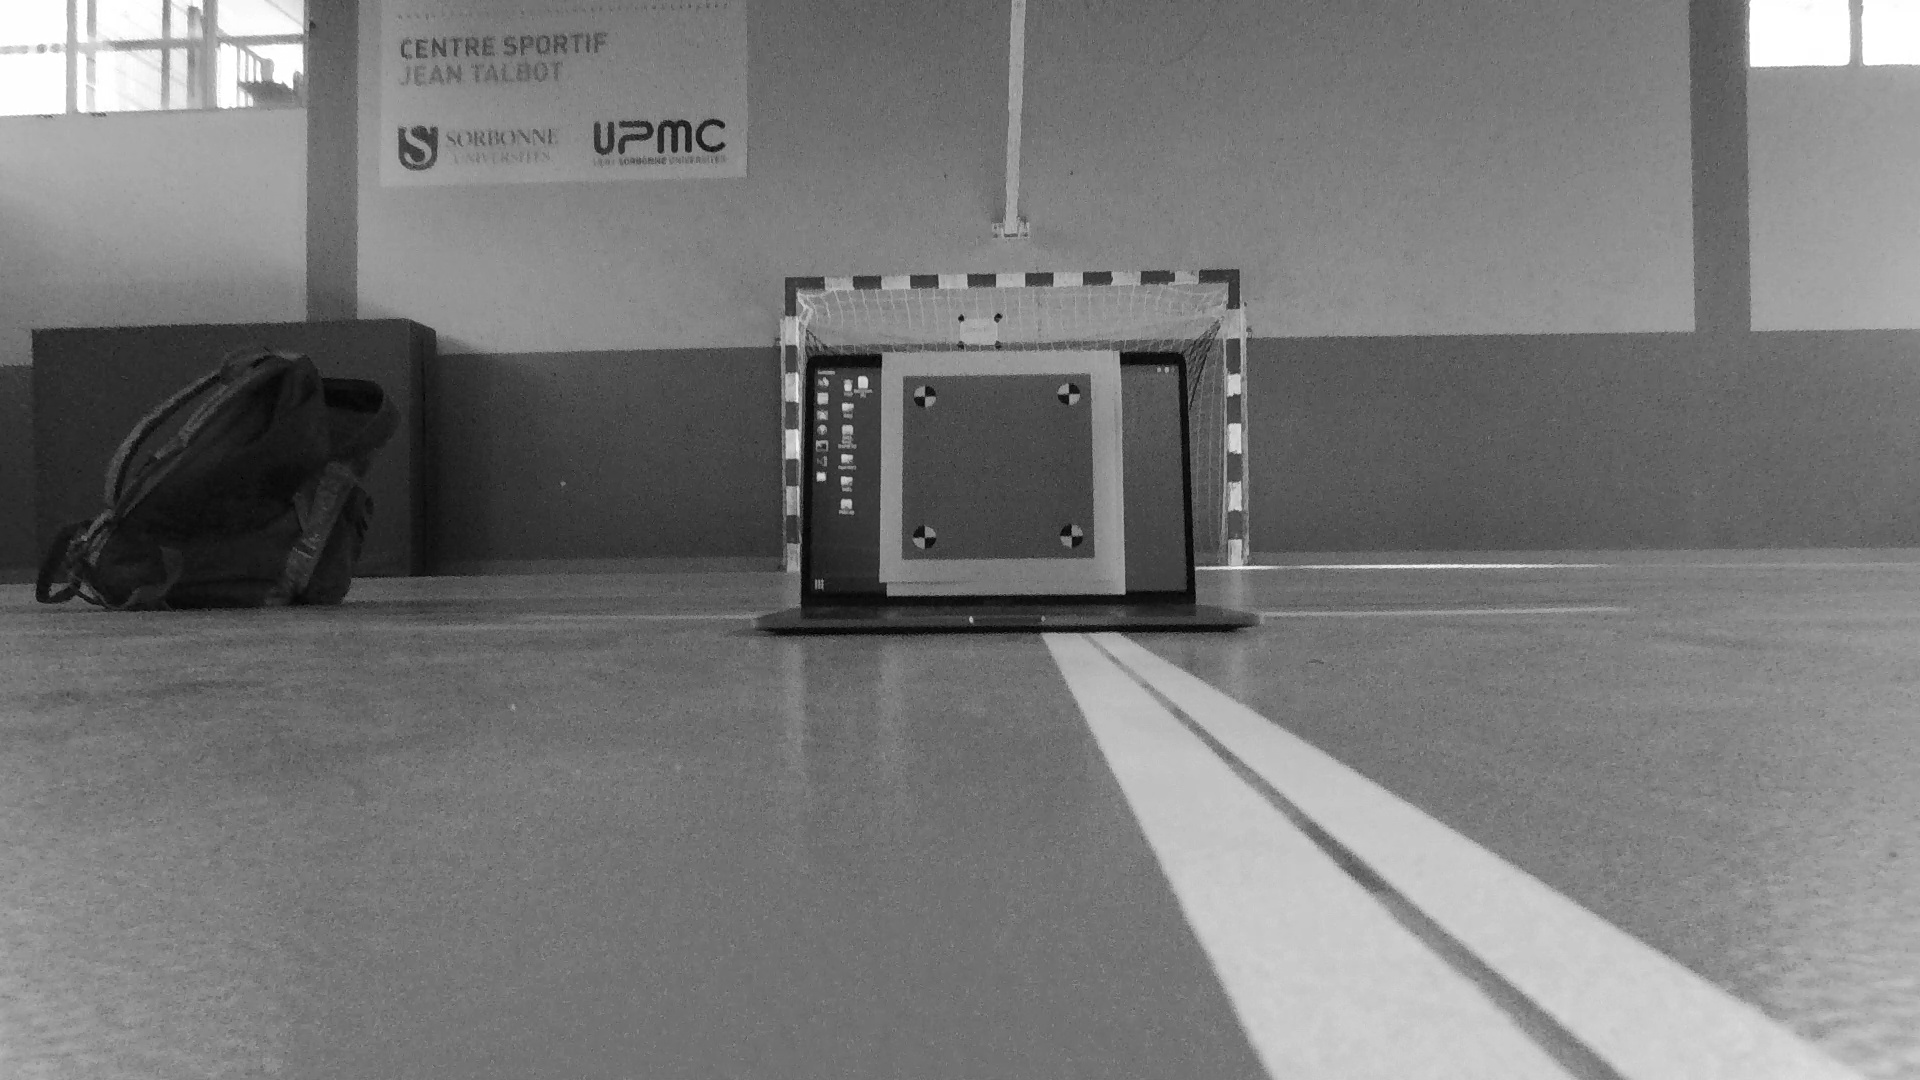
\includegraphics[width=5cm]{B_petits_cercles.jpg} }}
    \qquad
    \subfloat[Nouvelle mire
    ]{{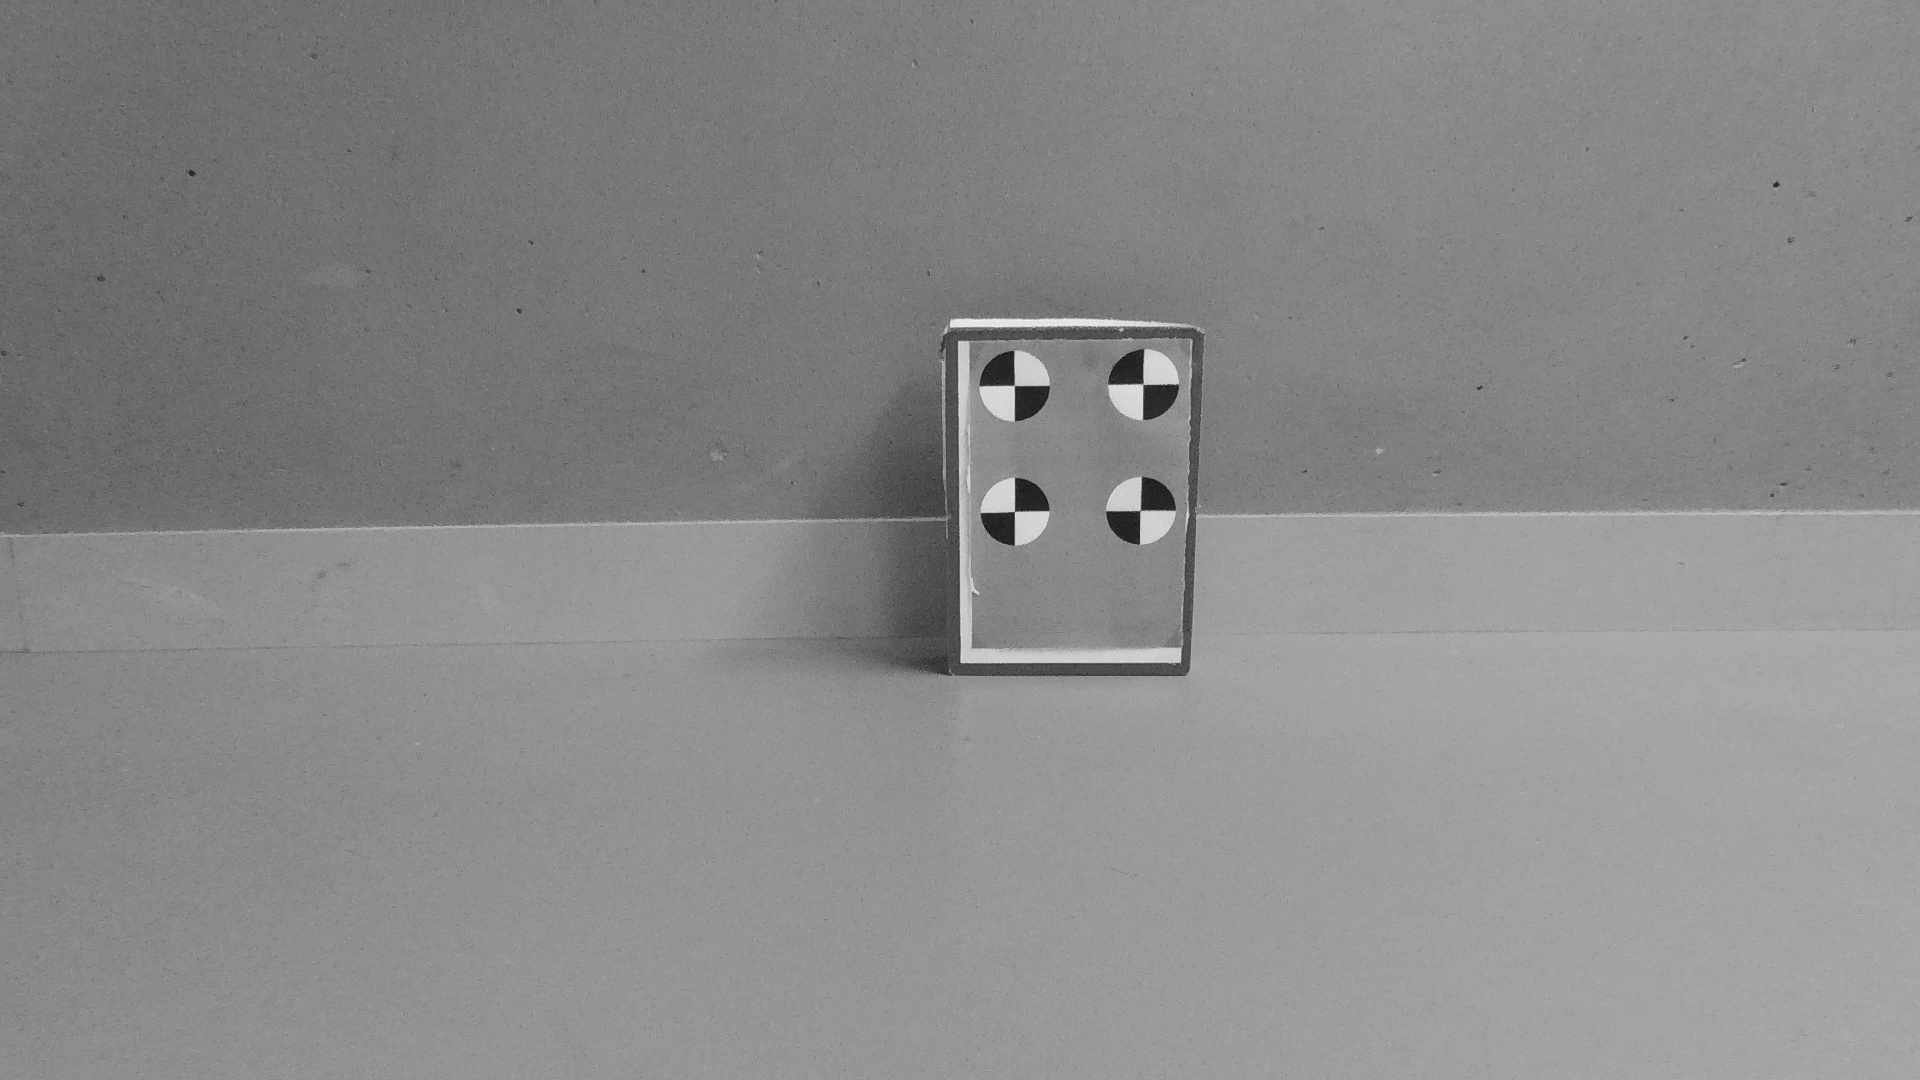
\includegraphics[width=5cm]{B_grands_cercles.jpg} }}
    \caption{Agrandissement du rayon des hirondelles.}
    \label{fig:rayon_mire}
\end{figure}

La figure ci-dessus (cf. Figure~\ref{fig:rayon_mire}) représente des images de vidéos prises avec le drone en le positionnant à la même distance de la mire (à 1 mètre).\\
Elle montre les deux mires utilisées dans ce projet. Nous pouvons constater même à l'oeil nu que nous avons du mal à repérer les centres de l'image de droite par rapport à la mire présentée à gauche.
\item \textbf{Latence : } 
le flux vidéo récupéré de la partie pilotage a une fréquence de 24 images/seconde. Le temps de réponse doit donc être inférieur à 1/24 = 42ms.\\
Pendant les tests, nous avons remarqué que la partie bas niveau à elle seule prenait un temps supérieur à 42ms.
La solution est de passer à 1 image sur deux, c'est à dire extraire l'image du flux 12 fois par seconde. Cela a réduit la latence mais le temps que prends cette partie est toujours très grand.

Il est très coûteux de calculer la somme des voisins pour chaque pixel des images. Pour éviter de tels calculs coûteux, le concept d'une \textbf{image intégrale \cite{image integrale}} (également connue sous le nom de table à aires additionnées) semble être une bonne alternative. Il utilise un moyen rapide et efficace pour calculer la somme des valeurs de pixels dans une image.\\
Dans l'image intégrale, la valeur en chaque point est déterminée en additionnant tous les pixels qui sont au-dessus et les pixels qui sont à gauche ainsi que le pixel cible lui-même (cf. Figure~\ref{fig:image_integrale}) .\\


\begin{figure}[H]
    \centering
     {{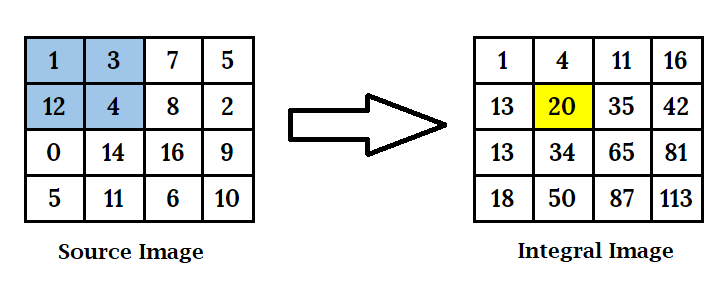
\includegraphics[width=10cm]{integral-image.png} }}
    \caption{Schéma explicatif du calcul de l'image intégrale.}
    \label{fig:image_integrale}
\end{figure}


Pour déterminer la somme des pixels sous un rectangle donné, nous utilisons l'image intégrale et n'exigeons que les 4 valeurs de coin au lieu de sommer tous les pixels sous-jacents individuellement. Donc, il y a une réduction significative du calcul car maintenant nous n'avons besoin que de 3 opérations et 4 valeurs de coin, quelle que soit la taille du rectangle (cf. Figure~\ref{fig:calcul_somme}).
\begin{figure}[H]
    \centering
     {{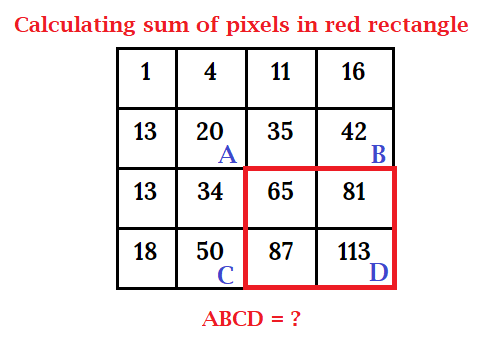
\includegraphics[width=10cm]{integral2.png} }}
     \caption{Schéma explicatif du calcul de la somme pour un pixel donné.}
    \label{fig:calcul_somme}
\end{figure}
La somme des pixels dans le rectangle ABCD peut être obtenue en utilisant les valeurs des points A, B, C et D, et cette expression D - B - C + A = 113 - 42 - 50 + 20 = 41 
Nous avons maintenant établi un moyen plus simple de calculer la somme/différence entre les sommes des valeurs de pixels de quatres rectangles, ce qui est parfait pour notre motif de calcul.

\item \textbf{Stratégies de robustesse : } dans le but d'augmenter l'efficacité de l'algorithme de détection,  
 nous avons décidé d'implémenter successivement deux stratégies.\\ 
 
En premier lieu, après avoir repéré les six meilleurs points de     
l'image, nous attribuons un score a chaque point  puis nous déterminons pour chaque point le nombre de points duquel il est espacé d'une distance supérieure à la distance maximum entre points.\\
Cette distance est variable en fonction des     
estimations de distances de la partie haute, ainsi si un point a un score supérieur ou égal a 3, qui veut dire qu'il est espacé d'au moins 3 points (point isolé), nous décidons de l'enlever car il est probablement éloigné du groupement de points qui constituent les hirondelles de la mire (cf. Figure~\ref{fig:strategie1}).\\

\begin{figure}[H]
    \centering
     {{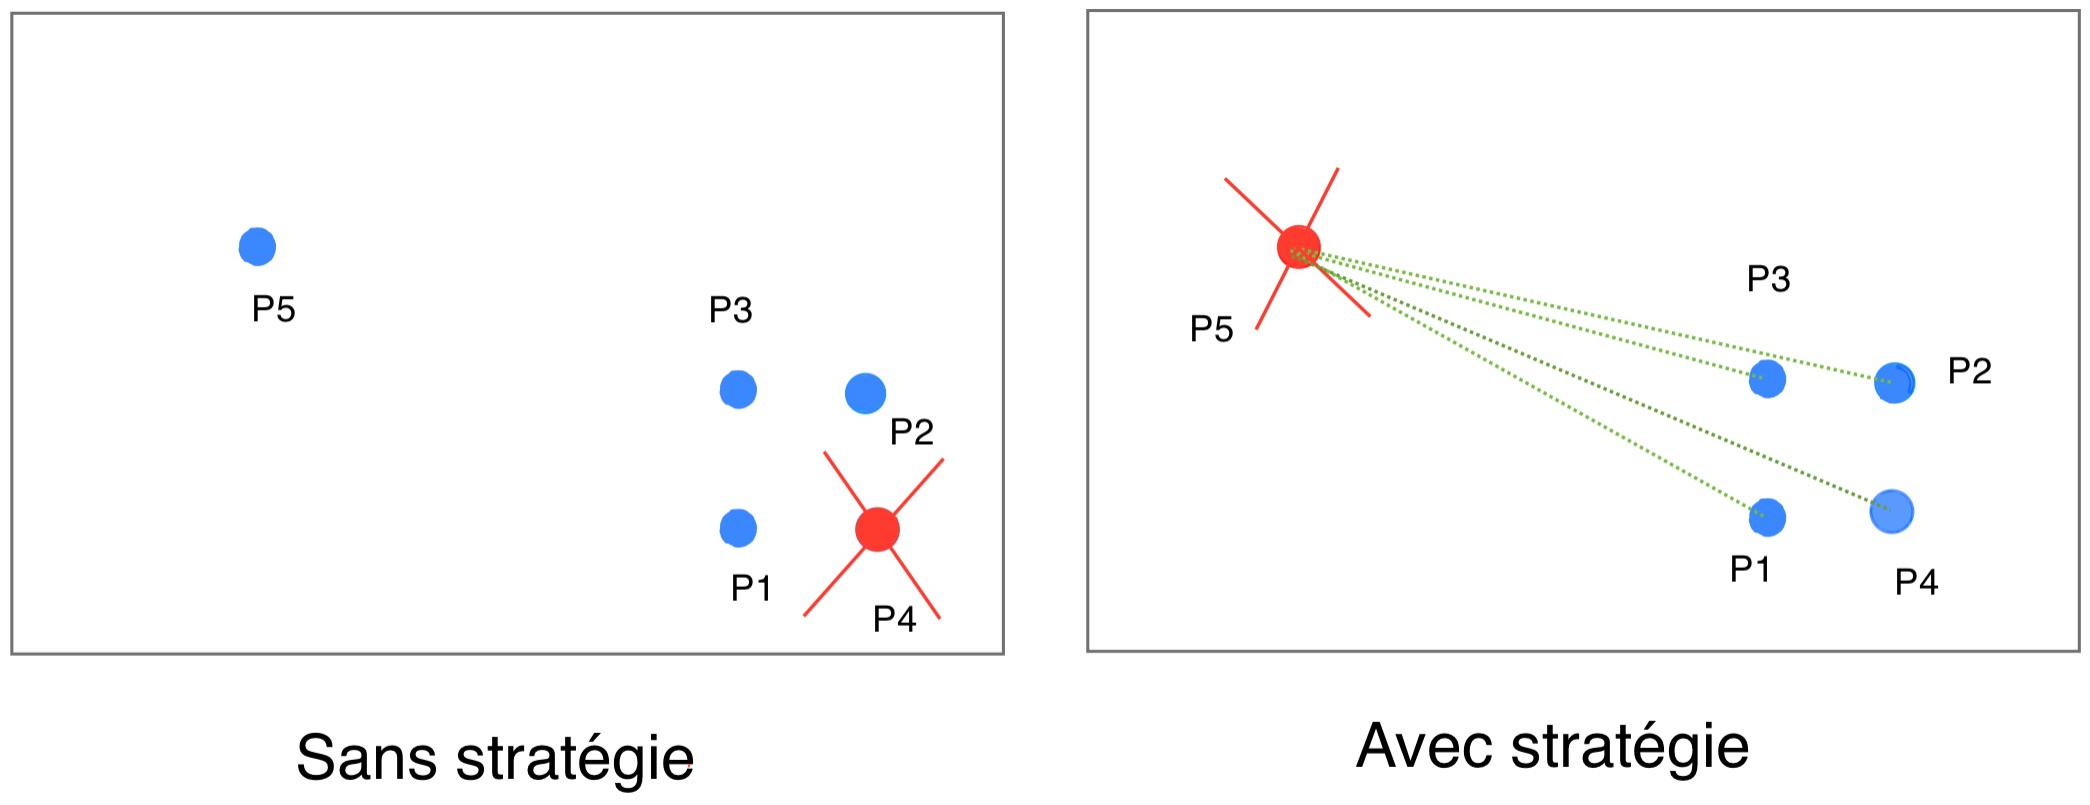
\includegraphics[width=13cm]{B_strategie1.png} }}
    \caption{Schéma explicatif du résultat obtenu en appliquant la première stratégie.}
    \label{fig:strategie1}
\end{figure}

La figure ci-dessus représente le résultat de l'algorithme qui peut se produire avec ou sans la stratégie des scores.
Soient P1, P2, P3, P4 et P5 des points repérés par l'algorithme de détection avec les sommes respectives S1= 1300, S2=1320, S3=1325, S4=1400 et S5=1380. Les points P1, P2, P3 et P4 représentent les centres des hirondelles de la mire. \\Sans appliquer la stratégie, le point P4 est éliminé car il est d'une somme supérieure aux quatre autres sommes des points.\\
En appliquant la stratégie, le point P5 est enlevé car il est distant du groupement des autres points.\\


La deuxième étape consiste à l'analyse des points restants, pour moins de trois points on met les valeurs des coordonnées du résultat à renvoyer à la partie haut niveau à -1, cela veut dire que les points n'ont pas pu être détectés.\\
Sinon, si on obtient trois points, on applique une fonction triangle qui permet de vérifier que les trois points forment un triangle.\\
Si on obtient quatre points alors on vérifie que les quatre points forment un quadrilatère (avec une marge de colinéarité variable).\\ Enfin si on obtient 5 ou 6 points alors on décide d'enlever les points dont la somme est supérieure aux autres points.  

\end{enumerate}

\subsection{Protocole expérimental}
Pour pouvoir tester notre programme avant de réaliser des tests sur le drone physique, nous avons utilisé des vidéos prises par le drone et par la caméra de notre ordinateur. Pour tester la validité du programme, nous appliquons l'algorithme de détection sur une vidéo, et nous observons les points retournés en dessinant un cercle sur l'image avec les coordonnées x,y retournés.

\paragraph*{Vidéos prises par le drone : }
nous avons utilisé dans un premier temps, les vidéos qui ont été prises par le drone pendant les séances de tests dans le centre Jean Talbot. Cela nous a permis de tester notre algorithme de détection. Néanmoins, en vue des scénarios possibles et des calibrages que nous avions besoin de faire ,ce n'était pas suffisant. 

\paragraph*{Vidéos prises par la caméra de notre ordinateur : }
en utilisant des outils de la bibliothèque FFmpeg, nous avons pu enregistrer des vidéos avec la caméra de notre ordinateur. Cela nous a été d'une grande utilité , car nous avions pu tester sur différentes compositions ( position initiale du drone, luminosité, distance de la mire ..etc).















\section{Imagerie de haut niveau\label{haut}}


\subsection{Objectif}
Dans cette partie, l’objectif consiste à estimer en continue la position du drone par rapport à la mire selon différents axes (cf. Figure \ref{fig:image1})  et évaluer son déplacement, afin de le faire atterrir devant la mire. \\ 
Les résultats de cette partie seront transmis à la partie pilotage qui sera chargée de les traduire en des commandes à transmettre au drone.
\begin{figure}[H]
\centering
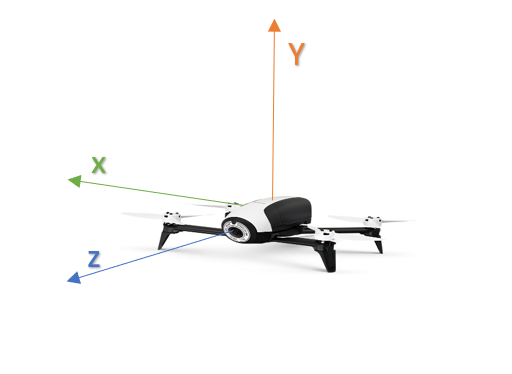
\includegraphics[height=3cm]{image1.PNG}
\caption{Drone et axes}
\label{fig:image1}
\end{figure}



\subsection{Entrée et sortie de la partie }
En entrée, cette partie reçoit des informations sur les coordonnées des hirondelles de la mire dans l'image, et en sortie, elle renvoie des estimations de la position du drone par rapport à la mire et si besoin une évaluation du mouvement. La sortie est sous forme d'une matrice d'entier de taille 4*2 où chaque ligne représente une estimation de la position sur un axe donné (X, Y, Z, Rotation).


\subsection{Réalisations de la partie}
\textbf{Pourquoi a-t-on besoin d’estimer la position et évaluer le déplacement ?} \\\\
Estimer la position du drone à chaque instant est le moyen le plus logique qui nous permet de savoir si le drone est proche de son objectif dans les meilleurs cas, mais aussi ça nous permet de le guider au mieux pour atteindre ce dernier dans le cas contraire.
Le drone n’est pas stable, il est exposé à son inertie, donc évaluer son déplacement à chaque instant nous permet de corriger très vite son déplacement avant de se retrouver très loin de son objectif ou de perdre ce dernier totalement du champ de vision de la caméra du drone. \\\\

\textbf{Comment?}\\\\
Les images capturées par le drone sont la seule information qui nous renseigne sur son environnement extérieur. Pour cela dans cette partie, on se base sur la position de la mire dans les images ainsi que des hypothèses qu’on pose. \\
Pour évaluer le déplacement du drone on compare sa position entre un instant t et un instant t-1.\\\\

\subsubsection{Estimer la position du drone}
    On utilise le principe de la logique floue \cite{LaLogiqueFloue} : c’est une méthode moderne de contrôle qui diffère de la logique classique. Elle était proposée par Zadeh en 1995. Elle nous permet d’exprimer différents niveaux, pas seulement vrai et faux.
    De ce fait, l'estimation de la position sur les différents axes du mouvement du drone (cf. Figure \ref{fig:lesAxes}) est réalisée par des automates d'états. Chaque état de l’automate représente une position possible du drone et chaque transition représente un mouvement possible.
    \begin{figure}[H]
            \centering
            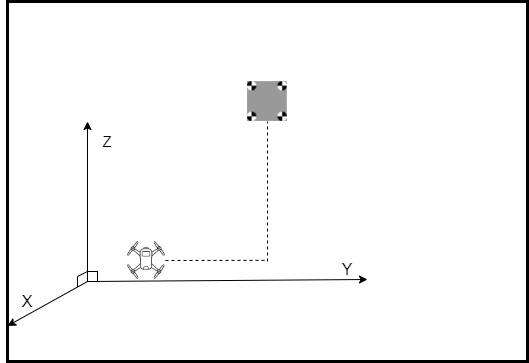
\includegraphics[height=4cm]{lesAxes.png}
            \caption{les axes}
            \label{fig:lesAxes}
            \end{figure}

    \begin{enumerate}
        \item \textbf{Estimation de la position sur l’axe des y} \\
           La position exacte du drone par rapport à la mire est très difficile à trouver, donc l’approche qu’on adopte est d’estimer à quel point le drone est proche ou loin de son objectif sur cet axe. Par conséquent, les mouvements ainsi que les positions possibles sont présentés dans l’automate sur la figure \ref{fig:image4}).\\
            \begin{figure}[H]
            \centering
            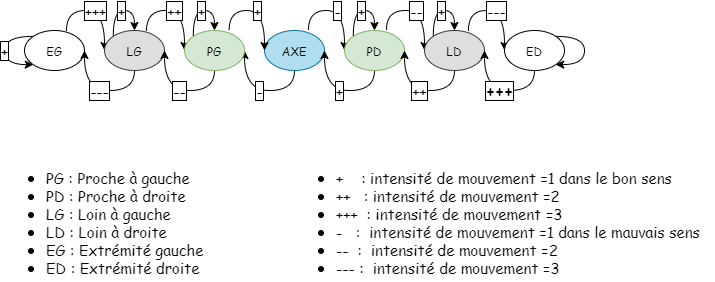
\includegraphics[height=4cm]{image4.png}
            \caption{Automate de l'axe Y}
            \label{fig:image4}
            \end{figure}
        
            Afin de déterminer cette position, on regarde celle de la mire dans les images reçues. En effet, il y a  une relation entre ces deux positions. Un exemple pour illustrer cette relation est exprimé dans la figure \ref{fig:image13}.\\
            \begin{figure}[H]
            \centering
            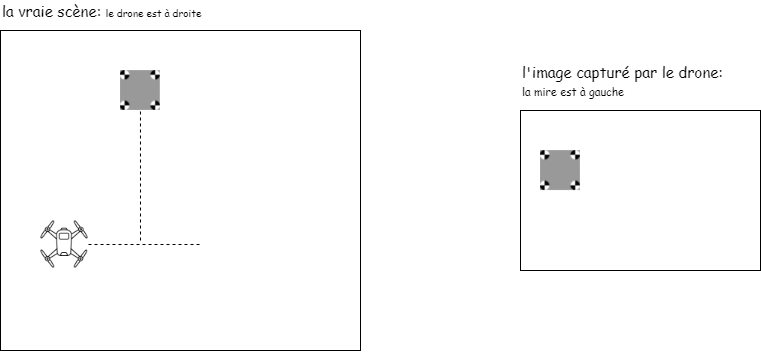
\includegraphics[height=5cm]{image13.png}
            \caption{la relation entre la position du drone et la position de la mire dans l'image}
            \label{fig:image13}
            \end{figure}
            Pour avoir la position de la mire, on estime sa distance au centre de l’image. La méthode utilisée pour cela était de diviser l’image en zones qui concordent avec les emplacements possibles que peut avoir le drone (cf. Figure \ref{fig:image2}).\\
            \begin{figure}[H]
            \centering
            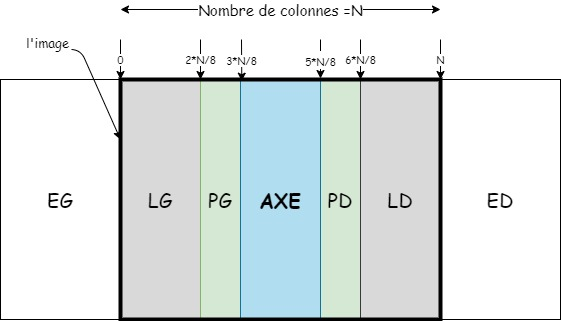
\includegraphics[height=4cm]{image2.jpg}
            \caption{La division de l'image par rapport l'axe des Y}
            \label{fig:image2}
            \end{figure}
            En recevant les coordonnées des hirondelles dans l’image, notre algorithme trouve la zone à laquelle appartient la mire. Ce résultat est interprété selon le tableau suivant:\\\\
            \begin{tabular}{|l|c|}
            \hline
            La zone à laquelle appartient la mire & L’interprétation\\
            \hline
            Très loin à gauche & Le drone est très loin à droite  \\
            Un peu loin à gauche & Le drone est un peu loin à droite \\
            Axe & Le drone est au centre \\
            Un peu loin à droite & Le drone est un peu loin à gauche \\
            Très loin à droite & Le drone est un très loin à gauche \\
            \hline
            \end{tabular}\\\\

            
        \item \textbf{Estimation de la position sur l’axe des X }\\
            La méthode pour estimer la position du drone sur l’axe des X est quasi similaire à celle utilisée sur l’axe des Y. 
            Les mouvements ainsi que les positions possibles sur cet axe sont présentés dans l’automate dans la figure \ref{fig:axeX}).\\
            \begin{figure}[H]
            \centering
            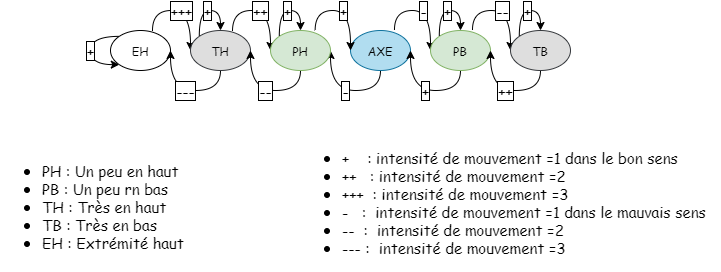
\includegraphics[height=4cm]{axeX.png}
            \caption{L'automate de l'axe X}
            \label{fig:axeX}
            \end{figure}
        
            Les images ont été divisées comme montre la figure \ref{fig:image3}.\\
            \begin{figure}[H]
            \centering
            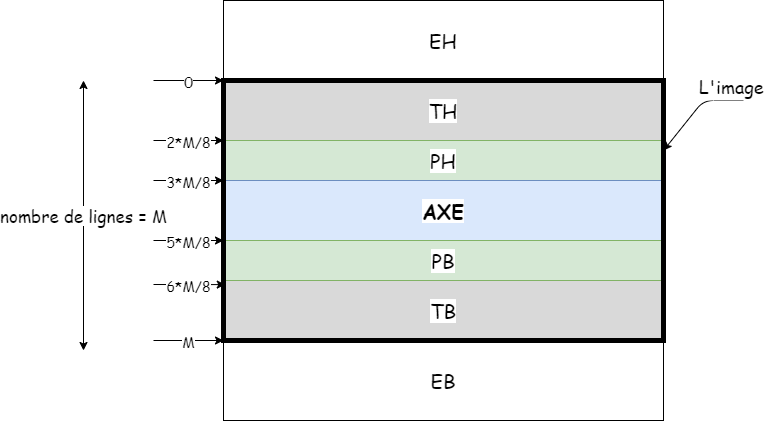
\includegraphics[height=4cm]{image3.png}
            \caption{ La division de l'image par rapport l'axe des x}
            \label{fig:image3}
            \end{figure}
            L'interprétation du résultat est faite selon ce tableau :\\\\
            \begin{tabular}{|l|c|}
            \hline
            La zone à laquelle appartient la mire & L’interprétation\\
            \hline
            Très en haut & Le drone est très en bas  \\
            Un peu en haut & Le drone est un peu en bas \\
            Axe & Le drone est au centre \\
            Un peu en bas & Le drone est un peu en haut \\
            Très en bas & Le drone est un très en haut \\
            \hline
            \end{tabular}\\\\
            
            
        \item \textbf{Estimation de la position sur l’axe des Z }\\
            Les mouvements ainsi que les positions possibles pour le drone sur cet axe sont représentés sur l’automate dans la figure \ref{fig:image6}).\\
            \begin{figure}[H]
            \centering
            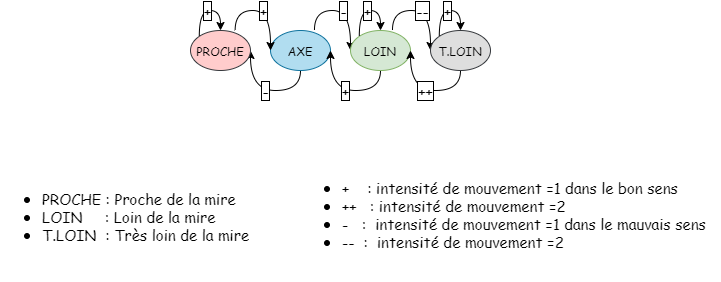
\includegraphics[height=4cm]{image6.png}
            \caption{L'automate de l'axe Z}
            \label{fig:image6}
            \end{figure}
        
            Afin de déterminer cette position, on regarde le nombre de pixels entre deux hirondelles de la mire. En effet, cette information nous renseigne sur la distance qui sépare le drone de la mire.\\
            À l’aide du calibrage réalisé à partir de différentes distances de la mire, les images ont été décomposées en zones. Avoir traité les mouvements selon cet axe uniquement si on a la mire au centre de l’image, nous assure avoir au moins 3 hirondelles renvoyées par la partie imagerie de bas niveau. Par conséquent, à chaque appel à notre partie, on calcule la différence entre les coordonnées selon l'axe des Y de deux hirondelles et on compare le résultat à la constante donnée par le calibrage pour estimer la profondeur du drone.
            La division de l’image en zones qui concordent avec les profondeurs possibles du drone est donnée dans la figure
             \ref{fig:image7}.\\
            \begin{figure}[H]
            \centering
            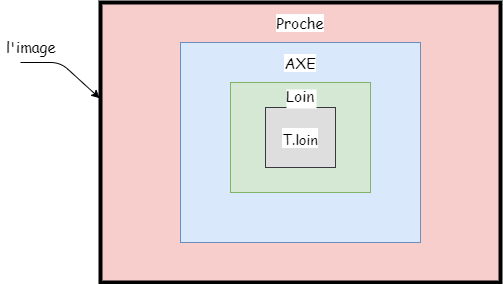
\includegraphics[height=5cm]{image7.png}
            \caption{La division de l'image par rapport à l'axe Z}
            \label{fig:image7}
            \end{figure}
            L'interprétation du résultat est faite selon ce tableau :\\\\
            \begin{tabular}{|l|c|}
            \hline
            La zone à laquelle appartient la mire & L’interprétation\\
            \hline
            Très loin & Le drone est très loin de la mire  \\
            Loin & Le drone est un peu loin de la mire\\
            Axe & Le drone suffisamment proche de la mire \\
            Proche& Le drone est très proche de la mire \\
            \hline
            \end{tabular}\\\\
            
        \item \textbf{Estimation de la position selon la rotation }\\
              L’approche qu’on a adoptée ici était d’estimer à quel point le drone est tourné par rapport à son axe de rotation. Par conséquent, les mouvements ainsi que les positions possibles sont présentés sur l’automate dans la figure \ref{fig:image19}).\\
            \begin{figure}[H]
            \centering
            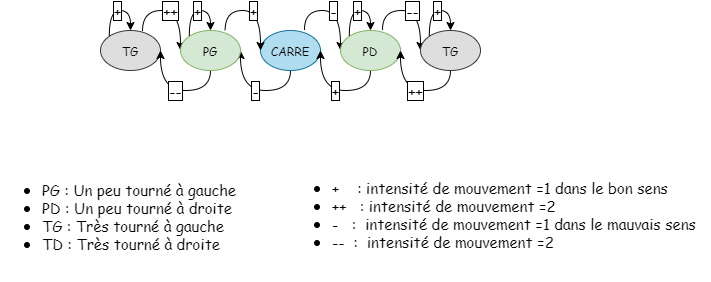
\includegraphics[height=4cm]{image19.png}
            \caption{L'automate de la rotation}
            \label{fig:image19}
            \end{figure}
            
            Afin de déterminer cette position, on regarde la déformation de la mire sur l'image reçue. En effet, la forme de la mire dans l’image nous renseigne sur le degré de rotation du drone (cf Figure \ref{fig:image9}).\\
            \begin{figure}[H]
            \centering
            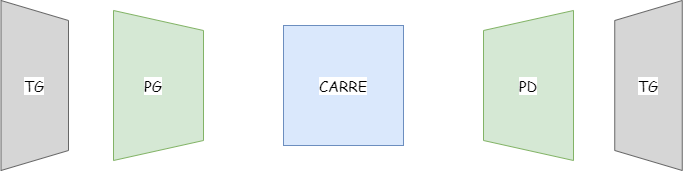
\includegraphics[height=2cm]{image9.png}
            \caption{La déformation de la mire}
            \label{fig:image9}
            \end{figure}
            Mais par contre la déformation de l’image possède un lien avec la profondeur du drone par rapport à la mire. Avec le même degré de rotation, une très petite déformation du drone à 3 m de la mire est équivalente à une très grande déformation du drone à 1 m de la mire, (cf. Figure \ref{fig:image10}). Ce qui nous oblige à faire des calibrages de chaque degré de rotation à toute distance possible entre le drone et la mire pour pouvoir quantifier le degré de rotation.
            Une solution qu’on a trouvé pour éviter ce problème était plutôt d'utiliser un rapport qu’on a appelé \textbf{rapport de déformation} qui lui dépend uniquement de l’angle de rotation quelle que soit la profondeur du drone (cf. Figure \ref{fig:image11}).\\
            \begin{figure}[H]
            \centering
            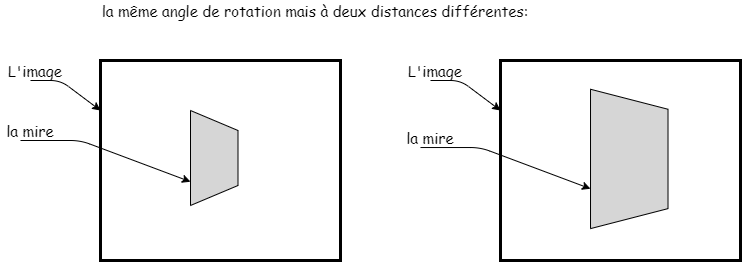
\includegraphics[height=4cm]{image10.png}
            \caption{La déformation de la mire avec un même degré à deux distances différentes}
            \label{fig:image10}
            \end{figure}
            \begin{figure}[H]
            \centering
            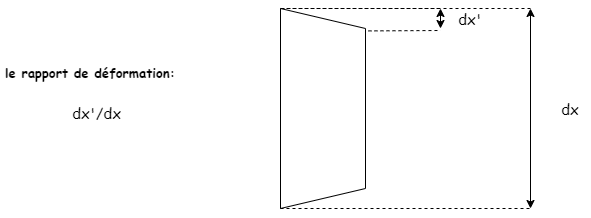
\includegraphics[height=4cm]{image11.png}
            \caption{Rapport de déformation}
            \label{fig:image11}
            \end{figure}
            
            Une rotation du drone est détectée par une déformation de la mire dans les images, mais il faut également fixer le sens de cette rotation. Pour cela on utilise les coordonnées de la mire sur l'image (cf. Figure \ref{fig:rotation}).\\ 
            
            \begin{figure}[H]
            \centering
            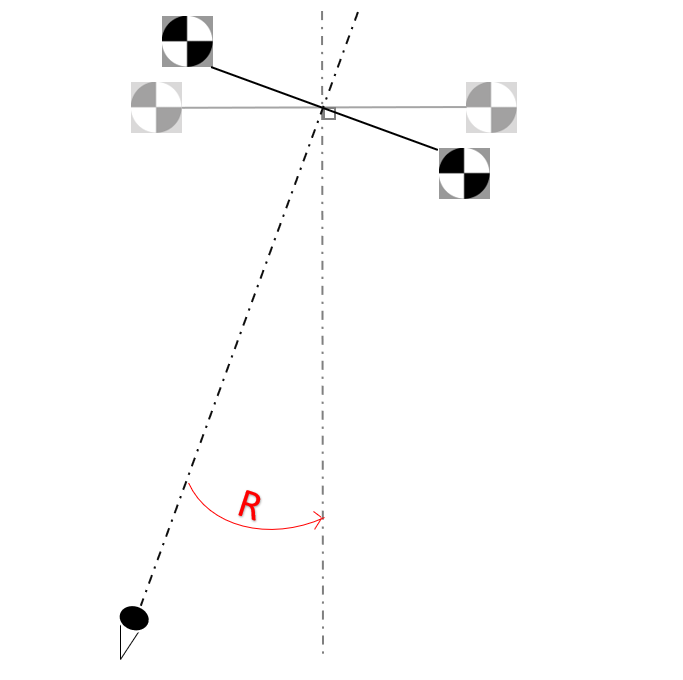
\includegraphics[height=4cm]{rotation.png}
            \caption{Le sens de rotation}
            \label{fig:rotation}
            \end{figure}
            
            L'interprétation du résultat est faite selon ce tableau : \\\\
            \begin{tabular}{|l|c|}
            \hline
            Le rapport de déformation & L’interprétation\\
            \hline
            Une très grande rotation à gauche & Le drone est très tourné à gauche \\
            Une petite rotation à gauche&Le drone est un peu tourné à gauche \\
            Pas de rotation & Le drone n’est pas tourné  \\
            Une petite rotation à droite & Le drone est un peu tourné à droite \\
            Une très grande rotation à droite  & Le drone est très tourné à droite\\
            \hline
            \end{tabular}\\\\
    \end{enumerate}
        
  
    
\subsubsection{Évaluation du mouvement du drone}
   Le but est d’éviter de perdre la mire de vue et aussi d’éviter de ramener le drone d’une position bonne à une position moins bonne (anticiper le mouvement).\\\\
    \textbf{Comment anticiper le mouvement ?}\\\\
    Pour évaluer le mouvement du drone on compare sa position à l’instant t à sa position à l’instant t-1 qu’on stocke comme historique. À chaque appel à notre fonction, on estime d’abord la position du drone, puis on accède à l'historique pour vérifier s’il est toujours dans le même état que précédemment, si c'est le cas, on regarde s’il avance vers l’état but ou non. S’il est toujours dans le même état que précédemment, si c'est le cas on regarde s’il avance vers l’état but. 

  \begin{enumerate}
      
 
        \item \textbf{Évaluation sur l'axe des X et Y }\\
        Le but est de ramener le drone devant la mire et par conséquent, cela revient à ramener la mire au centre de l’image. Un mouvement qui va avec cet objectif se caractérise par une distance entre la mire et le centre de l’image qui est décroissante. Donc, pour évaluer le mouvement du drone sur ces axes, à chaque appel à notre partie, si le drone se trouve toujours dans la même zone que précédemment, on calcule la distance dx et dy (cf. Figure \ref{fig:image14}). Si cette distance est plus petite que celle à l'état d'avant, on évalue le mouvement comme bon sinon mauvais .\\
        \begin{figure}[H]
        \centering
        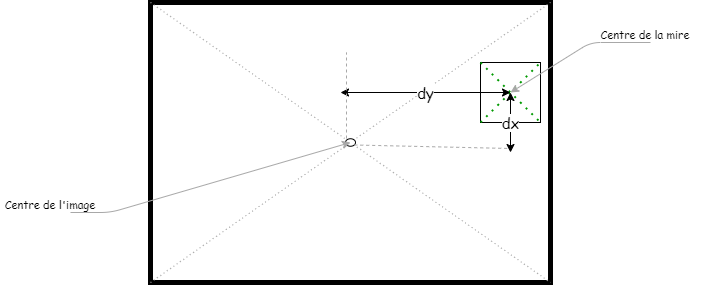
\includegraphics[height=4cm]{image14.png}
        \caption{l'évaluation sur X et Y}
        \label{fig:image14}
        \end{figure}
 
        \item \textbf{Évaluation sur l'axe des Z }\\
        De manière équivalente à celle précédemment, selon le sens du mouvement du drone, avance ou recule, le bon mouvement se caractérise par une différence entre les pixels des deux hirondelles de la mire qui augmente ou diminue (cf. Figure \ref{fig:image15}).
        \begin{itemize}
        \item Si on est loin et que la distance entre les deux hirondelles augmente on évalue le mouvement (avancer) comme bon sinon mauvais.
        \item Si on est très proche de la mire et que la distance diminue, on évalue le mouvement (reculer) comme bon sinon mauvais.
        \end{itemize}
        \begin{figure}[H]
        \centering
        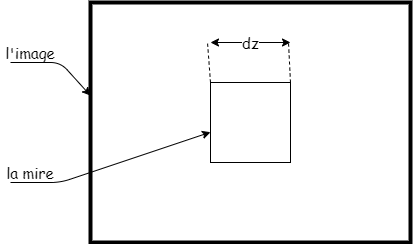
\includegraphics[height=3 cm]{image15.png}
        \caption{l'évaluation sur Z}
        \label{fig:image15}
        \end{figure}

        \item\textbf{Évaluation de la rotation }\\
         Évaluer un mouvement selon la rotation revient à comparer le degré de déformation dr (cf. Figure \ref{fig:image16})
        de la mire dans une image à l’instant t et à celui dans l’image à l’instant t -1. Si dr augmente, on évalue le mouvement comme bon sinon mauvais.\\
        \begin{figure}[H]
        \centering
        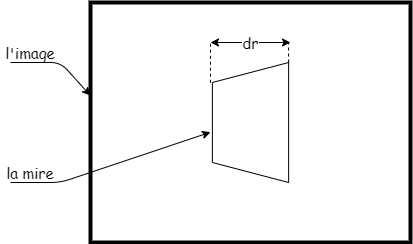
\includegraphics[height=3cm]{image16.png}
        \caption{l'évaluation de la rotation}
        \label{fig:image16}
        \end{figure}
        \end{enumerate}
  
  
   
\subsection{Les problèmes rencontrés et les solutions proposés}
\subsubsection{Manque et/ou absence d'informations}
  Parfois, la mire est partiellement repérée par la partie imagerie de bas niveau, par conséquent, il nous a fallu bien gérer ces cas afin d’assurer le bon fonctionnement du projet. C’est pourquoi on a généralisé nos algorithmes d’estimation de positions pour qu’il fonctionne même en recevant 0, 1, 2 ou 3 hirondelles au lieu de 4 ( toutes les hirondelles de la mire).


  
   \begin{itemize}
    \item Pour ce faire, tous nous algorithmes d'évaluation du mouvement et d’estimation de position sont capables de donner le bon résultat en recevant que 3 hirondelles, elles vérifient au début le nombre d’hirondelles reçues et par la suite à tout niveau de l’algorithme elles vérifient si une hirondelle est présente ou pas.
    \item Dans le cas où on reçoit 2 ou seulement une hirondelle on utilise l'historique pour déterminer l’estimation de position : par exemple, si on était très à gauche et par la suite, on a reçu que deux hirondelles à gauche notre algorithme estime que le drone est dans l'extrémité droite.
    \item Si on reçoit aucune information sur la mire on continue à envoyer la dernière estimation qui était faite, mais si on reçoit aucune nouvelle information au bout de 10 frames on informe la partie pilotage qu’on est perdu et qu’il faut recommencer dès le début et on réinitialise l'historique à 0.
    \end{itemize}
    
\subsubsection{Les risques de perdre la mire du champ de vision du drone}
Au démarrage, la mire se trouve dans le champ de vision du drone. Quand ce dernier se trouve à extrémité sur l'axe des Y, traiter la rotation peut engendrer la perte de la mire dans les images. Également quand le drone se trouve à l'extrémité sur l'axe des X, avancer peut aussi engendrer la perte de la mire. Afin de résoudre ce problème et minimiser le temps nécessaire au drone pour atteindre son objectif, on a décidé d’implémenter la stratégie (cf. Figure \ref{fig:image18}).
Dans cette stratégie, on donne la priorité pour l'axe des Y : une fois le drone est bien placé sur cet axe (l'état AXE de l'automate) on commence à traiter son déplacement sur l'axe des X. Une fois le drone est bien placer sur cet axe, on avance ou on recule pour le mettre dans l'état axe de l'automate Z. Une fois, on est à une bonne position sur les axes X et Y et à une distance suffisamment proche de la mire, on traite la rotation du drone. Un exemple du comportement du drone avec cette stratégie est donné dans la figure(cf. Figure \ref{fig:image17}). \\
\begin{figure}[H]
\centering
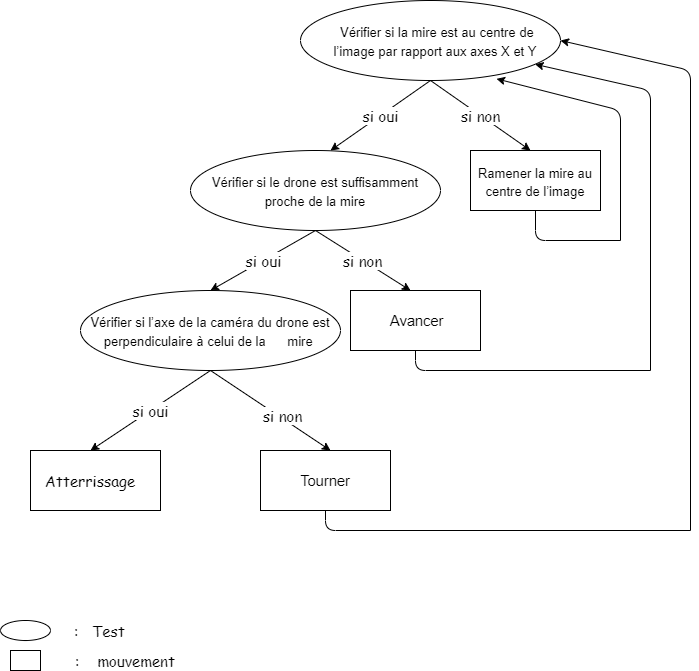
\includegraphics[height=8cm]{image18.png}
\caption{La stratégie implémentée}
\label{fig:image18}
\end{figure}
\begin{figure}[H]
\centering
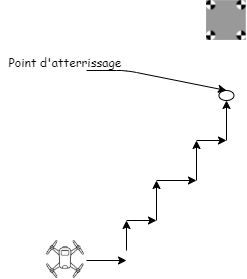
\includegraphics[height=5cm]{image17.png}
\caption{Le résultat de la stratégie}
\label{fig:image17}
\end{figure}
\subsubsection{La détection de la rotation}
Quand le drone est loin, la déformation de la mire peut ne pas être repérable. Ce qui nous a amené à quantifier la rotation uniquement dans le cas où le drone est suffisamment proche de la mire.
De plus, les constantes fixées par le calibrage de la rotation sont trop petites (le rapport de déformation) et comme la partie imagerie de bas niveau, ne parvient pas à nous renvoyer un carré parfait (décalage entre les x des hirondelles) même dans le cas d'absence de rotation, donc parfois notre algorithme détecte une petite rotation alors qu'y en a pas. 

\subsection{Protocole expérimental}
    Afin de vérifier le bon fonctionnement de cette partie, en premier lieu des analyses à la main, ont été faite sur les entrées et les sorties que renvoient nos algorithmes. En deuxième lieu des tests avec la partie imagerie de bas niveau, on était mis en place à l'aide de la caméra de l'ordinateur, ou le but été de vérifier le bon fonctionnement des deux parties ensemble. En troisième lieu, des essais sur le simulateur pour vérifier l'intégration de toutes les parties ensemble, et en dernier lieu, des séances d'essais sur le vrai drone, nous ont montré les bonnes et les mauvaises pratiques.

\section{Conclusion}
Dans ce rapport nous avons présenté les solutions et les scénarios de validation proposés par chaque partie. Nous avons pu construire et tester un premier modèle qui valide un scénario où la mire est en vue, et le drone effectue ses différents mouvement pour se mettre face à elle, s'avancer et enfin atterrir.
En guise de perspective, il serait intéressant d'augmenter la robustesse de la partie imagerie afin de pouvoir gérer le scénario où la mire n'est pas en vue. Quant à la partie pilotage, il serait intéressant d'affiner un peu plus les impulsions ,la correction de l'inertie du drone et d'augmenter la robustesse des mécanisme de protection du drone.
Nous avons pu validé grâce aux essais sur le drone et sur le simulateur le premier scénario où la mire était en vue. Des améliorations sont à prévoir pour les deux parties afin de gérer le deuxième scénario où le drone effectue d'abord la recherche de la mire avant d'effectuer les mouvements pour atterrir.

\newpage
\begin{thebibliography}{12}
\bibitem{git} 
Code source: \path{https://github.com/MRVNY/Projet-Drone}

\bibitem{pthreads}
pthreads:
\path{https://man7.org/linux/man-pages/man7/pthreads.7.html}

\bibitem{sphinx} 
Parrot Sphinx: \path{https://developer.parrot.com/docs/sphinx/whatissphinx.html}

\bibitem{SDK}
Parrot SDK3:
\path{https://developer.parrot.com/docs/SDK3/general-information}

\bibitem{alchemy}
Alchemy:
\path{https://github.com/Parrot-Developers/alchemy}

\bibitem{bebopsample}
BebopSample:
\path{https://github.com/Parrot-Developers/Samples/blob/master/Unix/BebopSample/BebopSample.c}

\bibitem{nmcli}
nmcli:
\path{https://linux.die.net/man/1/nmcli}

\bibitem{image integrale} 
Image intégrale: \path{https://medium.com/@anubhavroh/integral-image-141f6181db5e}

\bibitem{Calibrage}
Calibrage:
\path{http://www.optique-ingenieur.org/fr/cours/OPI_fr_M04_C01/co/Contenu94.html}
\bibitem{LaLogiqueFloue}
LaLogiqueFloue:
\path{https://www.techno-science.net/glossaire-definition/Logique-floue.html}


\iffalse
\bibitem{Commande référencée vision pour drones à decollages et atterrissages verticaux}
HAL : archive ouverte:
\path{https://hal.archives-ouvertes.fr/tel-01092388/document}
\fi

\bibitem{bebop}
Parrot Bebop 2:
\path{https://www.parrot.com/assets/s3fs-public/2019-01/parrotbebop2ledronetoutenun.pdf}

\bibitem{github}
gitHub: \path{https://github.com/}

\end{thebibliography}



\end{document}